\documentclass{article}

% -------------------- Packages --------------------
\usepackage{graphicx} % Required for inserting images
\usepackage{tabularx}
\usepackage{booktabs}
\usepackage[mode=text]{siunitx}
\usepackage{csquotes}\MakeOuterQuote{"}
\usepackage{xcolor}
\usepackage[
  colorlinks=true,
  linkcolor=blue,
  citecolor=blue,
  urlcolor=blue
]{hyperref}
\usepackage{soul}
\usepackage{placeins}
\usepackage[a4paper, margin=2.5cm]{geometry}
\usepackage{authblk}
\usepackage{booktabs}
\usepackage{tabularx}
\usepackage{dcolumn}
\usepackage{amsmath}
\usepackage{amssymb}
\usepackage{amsthm}
\theoremstyle{plain}
\newtheorem{proposition}{Proposition}
\newtheorem{corollary}{Corollary}
\usepackage{array}
\usepackage{threeparttable}
\usepackage{rotating}
\usepackage{tikz}
\usetikzlibrary{arrows.meta,positioning}
\newcolumntype{R}{>{\raggedleft\arraybackslash}X}

% -------------------- Bibliography --------------------
\usepackage[style=apa6,sortcites=true,sorting=nyt,backend=biber]{biblatex}
\addbibresource{references.bib}

\title{The Information Costs of Climate Misinformation: \\\large Evidence from Global Financial Data}
\author[1]{James Rice}
\affil[1]{Department of Government, University of Essex}
\date{\today}

\begin{document}
\maketitle

\begin{abstract}

Climate misinformation can alter the information environment in which investors and liquidity providers trade. This paper examines that relationship in a firm-day panel of 204 listed climate-transition firms from 2012 to 2025. The primary outcome is the percent quoted bid--ask spread, a measure of market liquidity and an observable proxy for information asymmetry. Sector-specific exposure is constructed by classifying English-language Facebook climate posts against nine energy sub-industries. The estimates compare within-firm changes, with firm and year-month fixed effects, controls for trading and macroeconomic conditions, and standard errors clustered by firm and calendar date. Greater exposure is associated with significantly wider quoted spreads, and the association strengthens at a one-day lag. Price impact does not move in the opposite direction, while rolling CAPM beta and Fama--French excess returns remain weak under two-way clustering. This pattern is inconsistent with liquidity fragility and more consistent with adverse-selection pressure.
\end{abstract}

\noindent\textbf{Keywords:} Climate Misinformation, Information Asymmetry, Market Microstructure, Environmental Communication, Politics and Governance, Corporate Responsibility.

\section{Introduction}

The information landscape surrounding climate change has been systematically distorted by misinformation campaigns (\cite{cobb2025politics}). Markets aggregate information, but they do so at a price. Climate misinformation is produced for political ends---funded by fossil-fuel interests, amplified by ideologically motivated actors, and timed to political events (\cite{farrell2016network}; \cite{oreskes2010merchants}; \cite{cinelli2021echo})---yet market-microstructure theory gives two opposing predictions for its effect on trading costs. If misinformation increases the advantage of sophisticated traders who can distinguish credible signals from false ones, liquidity providers should widen bid--ask spreads to protect themselves. If misinformation instead attracts uninformed retail trading, the perceived share of informed order flow may fall and spreads may narrow even as the market's capacity to absorb informed trading deteriorates. Which pattern prevails is the central question of this paper.

This question connects two related literatures. Political-behavior research shows that misinformation changes beliefs, trust, and collective action (\cite{flynn2017misperceptions}; \cite{bursztyn2020misinformation}), while climate-finance research shows that climate news, disclosure, and policy uncertainty are priced in financial markets (\cite{engle2020hedging}; \cite{bolton2021climate}; \cite{pankratz2023climate}). Neither literature traces the daily flow of politically produced climate misinformation into the mechanism that sets trading costs. Market microstructure provides that link because the quoted bid--ask spread is an observable price of information asymmetry and a direct measure of market liquidity (\cite{GlostenMilgrom1985}; \cite{EasleyOHara1992}).

The theory distinguishes two causal channels. Under adverse selection, false claims about climate science, carbon policy, and the viability of low-carbon technologies make the implications for fossil-fuel and renewable firms harder to assess. Traders able to verify those claims gain an informational advantage over those who cannot. Liquidity providers then face greater expected losses when trading climate-transition equities with better-informed counterparties and widen spreads, while price impact rises. Under liquidity fragility, viral climate-policy and energy narratives instead draw noise traders into the affected sub-industries. A larger uninformed share lowers the perceived probability that the next order is informed, narrowing the spread, but shallow order flow allows each dollar traded to move prices more, raising price impact. H1 tests the latter account: higher firm-day exposure to sector-specific climate misinformation should be associated with narrower percent quoted spreads and higher per-dollar price impact. Section~\ref{sec:theory} develops the mechanisms and their observable implications.

The empirical analysis uses 726,890 firm-day observations on 204 listed climate-transition firms from January 2012 to December 2025. The primary outcome is the percent quoted bid--ask spread; price impact supplies the second liquidity measure required for the joint test. Rolling CAPM beta and Fama--French five-factor excess returns serve as benchmark outcomes for systematic risk and return-pricing channels. The exposure measure is constructed by classifying 217,954 English-language Facebook climate posts from the Meta Content Library against nine TRBC energy sub-industries. Each firm inherits the exposure assigned to its sub-industry on each date, producing within-day cross-sectional variation while preserving the political and economic content of the posts.

Greater sector-specific misinformation exposure is associated with significantly wider quoted spreads after firm and year-month fixed effects, and the relationship strengthens at a one-day lag. Price impact does not display the divergence required by H1. The pattern is therefore inconsistent with liquidity fragility and more consistent with an adverse-selection response.

The paper makes three contributions. First, it extends market-microstructure theory to politically produced climate misinformation and distinguishes adverse selection from liquidity fragility through the joint behavior of spreads and price impact. Second, it provides a high-frequency firm-day exposure measure that maps political misinformation to the sub-industries whose values depend on the contested information. Third, it shows why inference requires within-day cross-sectional variation rather than a market-wide daily misinformation series. Together, these contributions connect the political production of misinformation to the liquidity of climate-transition equities without treating changes in risk or returns as the primary outcome.

The rest of the paper proceeds as follows. Section~\ref{sec:lit_review} reviews research on information and market liquidity and connects it to climate misinformation in financial markets. Section~\ref{sec:theory} develops the competing adverse-selection and liquidity-fragility mechanisms and states the hypothesis formally. Section~\ref{sec:data} introduces the firm-day financial panel and misinformation corpus. Section~\ref{sec:model} separates the market-liquidity design from the benchmark risk-and-return designs and sets out the identification and inference strategy. Section~\ref{sec:results} reports the main estimates, placebo, and robustness checks. Section~\ref{sec:discussion} interprets the findings, and Section~\ref{sec:conclusion} concludes.

\section{Literature Review}
\label{sec:lit_review}

\subsection{Information and Market Liquidity}

Market liquidity depends on the distribution and credibility of information. When some traders possess information that others lack, liquidity providers face the risk of trading at stale prices with better-informed counterparties (\cite{Akerlof1970}; \cite{GlostenMilgrom1985}; \cite{EasleyOHara1992}; \cite{Kyle1985}). They recover the expected loss through the bid--ask spread, while price impact records how strongly order flow moves prices. These measures make the trading-cost implications of information asymmetry observable. Costly information prevents markets from becoming fully efficient (\cite{GrossmanStiglitz1980}; \cite{Stiglitz2000}), and liquidity providers revise quotes as the perceived composition of informed and uninformed order flow changes (\cite{Hasbrouck1991}; \cite{easley1996}). Wider spreads indicate lower market liquidity and can pass through to firms' costs of capital (\cite{Tse2024}; \cite{Aliyev2025}; \cite{Aquilina2025}).

The credibility of public signals shapes this information environment. Financial disclosure lowers the cost of acquiring reliable information when investors regard the discloser as credible; weak or non-credible signals raise verification costs and the cost of capital (\cite{DiamondVerrecchia1991}; \cite{Verrecchia2001}; \cite{healy2001information}; \cite{LeuzVerrecchia2000}; \cite{BushmanSmith2001}; \cite{GoldsteinYang2017}). Investors' updates also depend on the perceived bias and authenticity of the source (\cite{Dye1985}; \cite{Cologna2022ValueJudgements}; \cite{KorehMandelkern2024}). Misinformation can therefore affect liquidity without changing firms' underlying cash flows: it degrades the public signal, increases the cost of separating credible information from false claims, and changes the risk that liquidity providers attach to incoming orders. Recent studies linking digital information and misinformation to liquidity document related effects on market microstructure (\cite{HerzingMuck2025}; \cite{DeesOzyurtMiller2026}; \cite{Mo2026ClimateRiskDisclosureMispricing}; \cite{LEIPPOLD202264}).

\subsection{Climate Misinformation and Financial Markets}

Climate misinformation is a politically produced distortion of that public signal. Organized campaigns by carbon-intensive industries have manufactured uncertainty about climate science and regulation, while partisan media and digital platforms amplify the resulting claims (\cite{oreskes2010merchants}; \cite{farrell2015corporate}; \cite{farrell2016network}; \cite{SupranRahmstorfOreskes2023}; \cite{VosoughiRoyAral2018}; \cite{acemoglu2010spread}). Exposure changes factual beliefs, hardens partisan misperceptions, erodes trust, and resists correction (\cite{flynn2017misperceptions}; \cite{NyhanReifler2010}; \cite{lewandowsky2017beyond}; \cite{bursztyn2020misinformation}; \cite{lazer2018science}; \cite{cobb2025politics}). Climate misinformation is a political problem because it distorts the evidence citizens use to evaluate policy proposals and hold decision-makers accountable. Organized interests can exploit uncertainty about climate science to weaken support for mitigation and delay regulation (\cite{farrell2019misinfo}). Understanding climate change requires interpreting long-term trends and probabilistic evidence; misleading arguments can exploit that difficulty by treating a cold weather event as a refutation of warming or uncertainty as evidence that action is unnecessary. \textcite{CookEllertonKinkead2018} show how such claims rely on faulty premises and reasoning. Confusion therefore need not reflect a simple absence of information: apparently plausible arguments and trusted partisan sources can make false claims persuasive. These studies establish the political and behavioral consequences of misinformation, but they do not show how the same content affects the liquidity of firms whose values depend on climate policy.

For businesses, these distortions can cloud expectations about regulation, demand for low-carbon products, and the returns to long-lived investments. That connection is plausible because climate-transition firms are unusually exposed to contested political information. Subsidies, carbon prices, disclosure requirements, and phase-out timetables are set through political institutions and international negotiations. Political and policy uncertainty carries a risk premium and raises volatility (\cite{PastorVeronesi2012}; \cite{PastorVeronesi2013}; \cite{BakerBloomDavis2016}), while partisan information and market sentiment can move prices independently of fundamentals (\cite{AZZIMONTI2023}; \cite{lei2023political}; \cite{DeLongShleiferSummersWaldmann1990}). Climate risk, news, and disclosure are likewise reflected in carbon premia, green-bond pricing, divestment, and institutional holdings (\cite{engle2020hedging}; \cite{bolton2021climate}; \cite{HongLiXu2019}; \cite{pankratz2023climate}; \cite{KruegerSautnerTangZhong2024}; \cite{flammer2021corporate}; \cite{FriedeBuschBassen2015}; \cite{Drahos_2025}). Misinformation differs from ordinary policy uncertainty because it corrupts the signal investors use to evaluate these exposures.

The verification problem is especially salient in fragmented climate governance, where public rules, transnational networks, private standards, taxonomies, and ratings offer competing signals whose authority can be politically contested or vulnerable to capture (\cite{KeohaneVictor2011}; \cite{HaleHeld2018}; \cite{Bodansky2016}; \cite{Rajamani2017}; \cite{AbbottSnidal2000}; \cite{ButheMattli2011}). Misinformation then makes genuine sustainability information harder to distinguish from greenwashing (\cite{delmas2011drivers}; \cite{marquis2016scrutiny}). The unresolved question is whether politically produced climate misinformation changes the trading costs through which markets process that information. The next section derives the competing liquidity predictions.

\section{Theory: Climate Misinformation and Market Liquidity}
\label{sec:theory}

The theoretical construct is information asymmetry: one party holds material information that another lacks (\cite{Akerlof1970}; \cite{Stiglitz2000}; \cite{StiglitzKosenko2024a}; \cite{StiglitzKosenko2024b}). The primary dependent variable is not information asymmetry itself, but the firm-day percent quoted bid--ask spread used to observe its liquidity consequences. In the sequential-trade model of \textcite{GlostenMilgrom1985}, a market maker posts a bid and an ask without knowing whether the next order comes from an informed or an uninformed trader. The spread compensates for expected losses to informed counterparties: the greater the perceived informed-trading risk, the wider the quote required to break even (\cite{EasleyOHara1992}; \cite{Hasbrouck1991}). A wider spread therefore indicates lower market liquidity and greater adverse-selection pressure.

Climate misinformation changes the public signal that investors use to value climate-exposed firms. Subsidy regimes, carbon prices, and regulatory timetables are political outcomes, and misinformation makes claims about those outcomes harder to evaluate (\cite{PastorVeronesi2012}; \cite{PastorVeronesi2013}; \cite{delmas2011drivers}; \cite{marquis2016scrutiny}). Investors differ in their ability and willingness to verify these signals. The resulting heterogeneity can affect trading through two competing microstructure channels.

Under the adverse-selection channel, sophisticated investors are better able to identify the credible climate-pricing signal, while less-informed investors are more likely to trade on false claims. This divergence increases the informational advantage of sophisticated traders. A liquidity provider who expects greater losses when orders originate from better-informed counterparties widens the bid--ask spread and quotes less depth. Per-dollar price impact should move in the same direction because trades reveal more private information. The observable prediction is therefore wider spreads and higher price impact, both indicating lower liquidity (\cite{grossman1980impossibility}; \cite{chordia2000commonality}; \cite{Han2022}; \cite{bordalo2020}). Here, sophistication refers to investors' capacity to verify information, not to a firm's climate performance. Larger or wealthier firms may nevertheless have better disclosure, stronger compliance capacity, and a more informed investor base, jointly affecting misinformation exposure and liquidity. Firm fixed effects and the market-capitalization control address stable firm differences and observed size changes, but do not eliminate time-varying differences in disclosure quality or regulatory preparedness. Figure~\ref{fig:theory_paths} summarizes the proposed adverse-selection pathway.

Under the liquidity-fragility channel, viral misinformation may divert attention from accurate information and attract inexperienced retail traders into climate-exposed stocks (\cite{barber2008all}; \cite{PengXiong2006}; \cite{sims2003}). If the uninformed share rises, the market maker's perceived probability that the next order is informed falls, narrowing the quoted spread. Yet this new order flow is shallow and noisy: each additional dollar traded moves the price by more, increasing price impact and weakening price efficiency. Liquidity fragility is this joint state in which trading appears cheaper at the quoted spread while the market's capacity to absorb informed flow deteriorates.

\begin{figure}[htbp]
\centering
\definecolor{pathnavy}{HTML}{173B57}
\definecolor{pathblue}{HTML}{EAF2F7}
\definecolor{pathgold}{HTML}{D8A547}
\definecolor{pathink}{HTML}{243746}
\begin{tikzpicture}[
  stage/.style={
    draw=pathnavy!60,
    fill=pathblue,
    rounded corners=2.2mm,
    align=center,
    text width=2.80cm,
    minimum height=2.65cm,
    inner xsep=2.5mm,
    inner ysep=3mm,
    font=\footnotesize,
    text=pathink
  },
  shock/.style={
    stage,
    draw=pathgold!85!black,
    fill=pathgold!14
  },
  outcome/.style={
    stage,
    draw=pathnavy,
    fill=pathnavy,
    text=white
  },
  flow/.style={
    -{Latex[length=2.5mm,width=1.7mm]},
    draw=pathgold!85!black,
    line width=0.9pt
  },
  node distance=0.42cm
]
\node[shock] (misinfo) {
  {\tiny\bfseries\color{pathgold!55!black}INFORMATION\\SHOCK}\\[4pt]
  \textbf{\mbox{Sector-specific}\\climate\\misinformation}
};

\node[stage, right=of misinfo] (signal) {
  {\tiny\bfseries\color{pathnavy!72}PUBLIC\\SIGNAL}\\[4pt]
  \mbox{Credible signals}\\\mbox{become harder and}\\\mbox{costlier to verify}
};

\node[stage, right=of signal] (risk) {
  {\tiny\bfseries\color{pathnavy!72}ADVERSE-SELECTION\\RISK}\\[4pt]
  \mbox{Liquidity providers}\\\mbox{expect greater losses}\\\mbox{to informed traders}
};

\node[outcome, right=of risk] (liquidity) {
  {\tiny\bfseries\color{pathgold!65}LIQUIDITY\\RESPONSE}\\[4pt]
  \mbox{Quoted bid--ask}\\\mbox{spreads widen and}\\\mbox{market liquidity falls}
};

\draw[flow] (misinfo) -- (signal);
\draw[flow] (signal) -- (risk);
\draw[flow] (risk) -- (liquidity);
\end{tikzpicture}
\caption{The adverse-selection pathway linking sector-specific climate misinformation to market liquidity.}
\label{fig:theory_paths}
\end{figure}

The first two pathways are distinguished by the sign pattern across the liquidity measures. Adverse selection predicts that quoted spreads and price impact widen together. Liquidity fragility predicts that they move apart: spreads narrow while price impact rises. H1 therefore states that \emph{higher firm-day exposure to sector-specific climate misinformation is associated with narrower percent quoted spreads and higher per-dollar price impact in the same firm-day panel.} The statistical test pairs the spread regression (Model~I) with a price-impact specification estimated on the same sample and with the same controls (Section~\ref{sec:results_priceimpact}). A widening spread, or the absence of the predicted divergence between the two measures, counts against H1.

Rolling CAPM beta and Fama--French five-factor excess returns provide benchmark outcomes rather than alternative measures of liquidity. A systematic-risk channel should appear in rolling beta (Model~II), whereas policy uncertainty, sentiment, or reduced confidence could appear in excess returns (Model~III; \cite{DeLongShleiferSummersWaldmann1990}; \cite{PastorVeronesi2012}). Under H1 these loadings should be small because a daily information shock changes the trading environment rather than firms' return covariances. The climate-finance literature further implies that any benchmark effect should be concentrated where climate news and disagreement are most relevant (\cite{engle2020hedging}; \cite{bolton2021climate}; \cite{HongLiXu2019}; \cite{pankratz2023climate}). The placebo, regional, and pre/post-2019 checks assess whether the observed pattern is specific to politically contested climate information rather than a general attention effect.

\section{Data}
\label{sec:data}

The unit of analysis is the firm-day. The estimation sample contains 726,890 firm-day observations on 204 listed climate-transition equities from January 2012 to December 2025. These firms---fossil-fuel incumbents and renewable challengers---are selected from a broader 19,183,738-firm-day universe using nine TRBC energy sub-industries. The financial panel supplies the liquidity outcomes, benchmark outcomes, and controls from Refinitiv Workspace, FRED, the World Bank, and the Kenneth French Data Library. The climate-misinformation corpus supplies the 217,954 unique English-language Facebook posts used to construct the exposure measure; each post's creation date matches at least one trading day in the panel. Appendix Tables~\ref{tab:panel_g}--\ref{tab:panel_n} and~\ref{tab:qwen_type} describe the corpus and its classifications, and Appendix Tables~\ref{tab:panel_a}--\ref{tab:panel_f} summarize the financial panel, its regional and temporal coverage, and the principal variables. All processing and merging is implemented in Python, and the replication code follows the transparency standards of \textcite{ChristensenMiguel2018}.

\subsection{Financial Panel and Outcome Measures}
\label{sec:data_financial}

The financial data come from a firm-level panel of 204 listed climate-transition equities sourced from Refinitiv Workspace via the Eikon Python API. The sample is defined by membership in one of nine TRBC energy sub-industries that span the fossil-fuel value chain (Coal, Integrated Oil \& Gas, Oil \& Gas Drilling, Oil \& Gas Exploration and Production, Oil \& Gas Refining and Marketing, Oil \& Gas Transportation Services, Oil Related Services and Equipment) and the renewable transition (Renewable Energy Equipment \& Services, Renewable Fuels). Listing regions cover China (CN), the European Union (EU), Japan (JP), the United Kingdom (UK), and the United States (US). For each security, identified by its RIC code, and each trading day, the panel records open, high, low, and close prices; trading volume and turnover; market capitalization; and dividend yield. Trade-level microstructure variables come from the Refinitiv tick-history database: bid--ask quotes, the volume-weighted average price (VWAP), intraday price moves, buyer- and seller-initiated trade counts, order flow, trade intensity, the bid--ask spread in levels and percent, intraday volatility, and price impact (\cite{Karpoff1987}; \cite{Parkinson1980}). The percent quoted spread---the bid--ask spread divided by the quote midpoint and expressed in percent---is the primary liquidity outcome. Price impact is the companion liquidity outcome required for the joint test of H1. Rolling CAPM beta and Fama--French excess returns provide the benchmark risk and return outcomes. The analysis focuses on climate-transition firms because their cash flows are directly exposed to climate policy and the energy transition that the misinformation corpus contests.

One practical concern is timing. The Shanghai trading day (UTC+8) ends before the New York session (UTC$-$5) begins, so a same-day merge assigns some misinformation activity that post-dates the Asian close to Asian-market outcomes. The one-day-lag specification in Table~\ref{tab:v2_lag}, estimated on the common firm-day sample, reduces this alignment concern by relating exposure on date $t$ to the next observed trading day. Static firm characteristics---exchange code, TRBC industry classification, country of headquarters, instrument type, and company name---are merged at the security level and are time-invariant within the panel. Region assignments come from RIC suffixes encoding the primary listing exchange, verified against Bloomberg and WRDS definitions for a random subsample of 1,000 firms (99.2\% agreement).

Macroeconomic controls come from the FRED API for the United States and the World Bank API elsewhere: GDP growth, unemployment, and CPI inflation for each region (\cite{FederalReserveBankofStLouis2025}; \cite{WorldBank2025}). Because many of these series are annual or quarterly, I forward-fill them to the daily panel:
\begin{equation}
M_{r,d} = M_{r,q(d)}, \quad \text{where } q(d) = \max \{q : \text{start}(q) \leq d\},
\end{equation}
so that each firm-day observation carries the most recent available value (\cite{StockWatson2008}). The interpolated macro panel merges with the firm-level data on calendar date and region, with full coverage for all three controls.

Daily Fama--French five-factor returns---market excess return (MktRF), size (SMB), value (HML), profitability (RMW), and investment (CMA)---come from the Kenneth French Data Library.\footnote{Data available at \url{https://mba.tuck.dartmouth.edu/pages/faculty/ken.french/data_library.html}.} I download six regional factor sets (US, Global, Europe, Japan, Asia Pacific ex-Japan, and North America) and match each firm by listing region and country of headquarters; the match fills 99.0\% of the panel. The risk-free rate ($R_f$) comes from the corresponding regional factor file and is used to compute daily excess returns.

Three variables are constructed from the raw panel. The daily simple return is
\begin{equation}
R_{i,t} = \frac{P_{i,t} - P_{i,t-1}}{P_{i,t-1}} \times 100,
\end{equation}
where $P_{i,t}$ is the closing price of firm $i$ on day $t$. The daily excess return is $R^e_{i,t} = R_{i,t} - R_{f,t}$, where $R_{f,t}$ is the regional daily risk-free rate from the Fama--French data. The rolling CAPM beta comes from 252-trading-day rolling OLS regressions of firm excess returns on the regional market excess return, requiring a minimum of 126 observations per window:
\begin{equation}
\hat{\beta}_{i,t} = \frac{\text{Cov}(R^e_{i,s}, \text{MktRF}_s)}{\text{Var}(\text{MktRF}_s)}, \quad s \in [t-251, t].
\end{equation}

The rolling beta is available for 71.9\% of the panel, with a mean of 0.54 and a median of 0.47. This mean sits below the 0.8--1.2 range typical of US equities, for three reasons. The sample is dominated by Chinese (mean $\beta = 0.66$) and Japanese (mean $\beta = 0.42$) firms, where thin trading and non-synchronous price adjustment bias OLS betas downward (\cite{ScholesWilliams1977}; \cite{Dimson1979}). Within the US subsample the mean is 0.49, pulled down by small-cap firms in the lower market-capitalization quintiles. And the rolling window screens out only the most thinly traded firms; applying the \textcite{Dimson1979} lead--lag correction would likely raise the mean toward conventional levels. Appendix Table~\ref{tab:beta_region_mktcap} reports mean betas by region and market-capitalization quintile.

The merged climate-transition panel is uniquely indexed by security and date, with no duplicates. China contributes the largest share of firm-day observations, followed by the United States and Japan, and panel composition is stable from 2012 through 2025. Appendix Table~\ref{tab:energy_desc_coverage} reports the composition and coverage of the 204-firm climate-transition sample.

Finally, the climate-transition panel is merged on calendar date and firm sub-industry with the firm-day misinformation-exposure index built from the Meta Content Library, described in Sections~\ref{sec:data_misinfo} and~\ref{sec:LLM} below. The main regressions use $\mathrm{Exp}^{\text{mean}}_{i,t}$ as the headline regressor of interest, with $\log(1+\mathrm{Exp}^{\text{sum}}_{i,t})$, $M^{\text{mean}}_{i,t}$, and $R^{\text{mean}}_{i,t}$ as variant specifications, all defined in Section~\ref{sec:LLM}.

\subsection{Climate Misinformation Corpus}
\label{sec:data_misinfo}

The misinformation measure is built from 217,954 unique English-language public Facebook posts---the subset of a 265,652-post corpus extracted from the Meta Content Library (MCL) whose Meta-recorded creation date matches at least one trading day in the climate-transition panel. The corpus was assembled through keyword searches across eight thematic datasets covering climate adaptation, climate politics, global climate justice, resilience, climate activism, and ecological themes; the posts span December 2009 to October 2025 and come from a long-tailed distribution of pages and profiles. Each post carries platform-reported engagement counts---likes, shares, comments, total reactions, and views---plus metadata on content type, surface type, and owner characteristics. Appendix Table~\ref{tab:panel_g} reports summary statistics on the corpus as a whole.

The corpus is an English-language, keyword-selected sample of public content, not a representative sample of national Facebook use. The available summaries do not establish the countries of origin of posts or the geographic distribution of their audiences, so differences in platform access, language, and user composition cannot be separated from differences in misinformation production. The exposure measure instead treats Facebook as a potential transnational information environment: claims about energy technologies, carbon policy, or fossil-fuel demand can circulate across borders and inform investors trading firms in the same sub-industry. For example, a claim originating in India could matter for a French-listed company if it reaches that company's investors or concerns markets or technologies relevant to its cash flows. The link is shared sector relevance and possible cross-border circulation, not the automatic transmission of every foreign post to every firm. The index measures the availability of relevant content, rather than observed investor attention or a country-to-country transmission effect.

The corpus enters this paper at the level of individual posts. Each (post, sub-industry) pair is scored by a single large language model on two continuous 0--100 scales---sector relevance and climate-or-energy misinformation---as described in Section~\ref{sec:LLM}; the firm-day index used in the empirical models is built from those scores. Three properties of the corpus matter for the analysis. First, the corpus is heavy-tailed in volume by year, with English-language climate-post volume more than tripling after 2019 (Appendix Table~\ref{tab:panel_j}). Second, the corpus is concentrated in supply: a small set of high-volume pages and profiles produces a large share of total posts (Appendix Table~\ref{tab:panel_l}), and platform-reported engagement counts are themselves heavy-tailed, with the highest-engagement posts diffusing on the order of three times the mean shares of the median post---a pattern consistent with the finding that misleading content travels disproportionately (\cite{VosoughiRoyAral2018}). Third, the corpus mixes climate-scientific content, climate-political content, and climate-adjacent content that is on-topic for some sub-industries and entirely off-topic for others; the firm-day construction in Section~\ref{sec:LLM} is what makes the sub-industry partition operational.

The classifier uses an open-weight model, and the post-level classifications and firm-day index built from them are released with the replication package. The raw post text falls under the MCL terms of use and is not redistributed. The classifier is assessed with a held-out spot-check (Section~\ref{sec:LLM}) rather than a hand-coded gold-standard sample (\cite{grimmer2022text}). Constructing a gold standard is less straightforward than for a binary label because the task requires two continuous 0--100 judgments---sector relevance and climate-or-energy misinformation---over nuanced content. A hand-coded benchmark would nevertheless provide a valuable direction for further measurement validation.

\subsection{LLM Classification of Misinformation}
\label{sec:LLM}

This section describes the classification framework that turns the corpus into a firm-day measure of misinformation exposure (\cite{WardleDerakhshan2017}). The design goal follows directly from the inference problem in Section~\ref{sec:model}: a regressor that is to vary across firms within a calendar day must be built by asking, for every post, a separate question of every sub-industry the panel contains. That is what the classifier does. It is called once on each of the 1,959,707 (post, sub-industry) pairs---each of the 217,954 paired posts judged against each of the nine TRBC energy sub-industries---and returns, for each pair, how relevant the post is to that sub-industry and how much climate-or-energy misinformation it contains. A market-wide daily index that collapsed a model's per-post scores into one number would, by construction, assign every firm the same value on a given day and reinstate the firm-invariant problem this paper is designed to avoid; only the per-sub-industry judgment produces the cross-sectional variation the design needs.

A single high-capacity model is used rather than an ensemble. At 1.96 million judgments, the 35-billion-parameter model can distinguish sincere false claims from satire and sector-relevant claims from off-topic content without the prohibitive runtime cost of repeated ensemble inference. Automated detection systems are themselves vulnerable to adversarial manipulation and raise ethical concerns (\cite{QiuLiuZhou&Huang2022}; \cite{HorneNevo&Smith2023}), so the design relies on one locally hosted, deterministic classifier whose outputs are reproducible bit-for-bit and whose rubric is fixed in advance and made explicit below.

The model is \texttt{Qwen3.6-35B-A3B-FP8}, a mixture-of-experts model with 35 billion total parameters and approximately 3 billion active parameters per token, served in 8-bit floating-point precision on a single NVIDIA Grace--Blackwell GB10 system-on-chip running the vLLM 0.21 inference engine. Inference uses temperature zero and structured-JSON grammar enforcement via the \texttt{xgrammar} backend, so each (post, sub-industry) judgment is deterministic, schema-valid, and reproducible (\cite{westwood2025measuring}; \cite{gilardi2023chatgpt}; \cite{santurkar2023whose}). Each judgment receives the firm's sub-industry profile (industry name, the set of countries and listing regions of firms in that sub-industry, and a list of example firm names) and the post (text, date, content type, link-attachment caption and description). The rubric instructs the model to score two continuous 0--100 quantities: \emph{sector relevance} $R_{p,s}$, capturing how materially the post's content relates to firms in sub-industry $s$, and \emph{climate-or-energy misinformation} $M_{p,s}$, capturing the degree to which the post contains false, misleading, or pseudoscientific claims about climate science or energy.

Two features of the rubric matter. First, misinformation is bounded to climate or energy claims. A post that contains political conspiracy theories unrelated to climate---antisemitic content about EU politicians, anti-vaccination conspiracies, electoral fraud claims---scores $M_{p,s}=0$ regardless of how false those other claims are; the score is a measure of climate-misinformation exposure, not a general misinformation index. Second, satire and parody are bounded to be not misinformation. A sarcastic Facebook post mocking climate denial that begins ``MDPI, the predatory journal of which nothing can be believed, according to Facebook climate experts'' is correctly classified at $M_{p,s}=0$ with the rationale ``satirical parody mocking climate denialism, not a sincere assertion of false claims''. These features were added to the rubric after a held-out spot-check on the first 2,000 judgments revealed that a default rubric over-scored political and parody content; the spot-check is reported in Appendix~\ref{sec:firmday_validation}.

The per-post composite exposure index is
\begin{equation}
\mathrm{Exp}_{p,s} \;=\; \frac{R_{p,s}\,M_{p,s}}{100},
\label{eq:exposure_post}
\end{equation}
on a 0--100 scale, which is non-zero only when the post is sector-relevant for sub-industry $s$ \emph{and} contains climate or energy misinformation. The product, rather than either factor alone, is the object of interest because the economic channel requires both: a false climate claim that has nothing to do with coal does not change what a coal trader needs to price, and an accurate, highly relevant post about coal carries no misinformation for the market to misprice. The index isolates the intersection---misinformation that is \emph{about} the firm's sector. The firm-day regressor used in the empirical models is the mean of this composite across the day's paired posts, evaluated at the firm's sub-industry:
\begin{equation}
\mathrm{Exp}^{\text{mean}}_{i,t} \;=\; \frac{1}{|P_t|}\sum_{p \in P_t} \mathrm{Exp}_{p,\,s(i)},
\label{eq:exposure_firmday}
\end{equation}
where $P_t$ is the set of climate posts whose Meta-recorded creation date matches calendar date $t$, and $s(i)$ is the TRBC sub-industry of firm $i$. Two volume-style variants enter the robustness checks: $\mathrm{Exp}^{\text{sum}}_{i,t}=\sum_p \mathrm{Exp}_{p,s(i)}$ (sensitive to the number of climate posts a firm's sector sees on a given day) and $\log(1+\mathrm{Exp}^{\text{sum}}_{i,t})$ (which tames the right skew). The raw components $R^{\text{mean}}_{i,t}$ and $M^{\text{mean}}_{i,t}$ are also persisted, to test whether the composite or one of its constituents carries the signal.

Three properties of the regressor matter for the inference design. First, two firms in different sub-industries on the same date receive different exposures: the model evaluates each post against the specific sub-industry, so a Renewable-Fuels firm and a Coal firm on the same trading day inherit different scores from the same set of posts. Second, two firms in the \emph{same} sub-industry on the same date share a value by construction; the level of aggregation at which the model is asked to reason is the sub-industry, not the firm. Firm-level fixed effects in the empirical models absorb the constant level of exposure that any firm experiences over the sample, leaving within-firm between-day variation as the identifying contrast. Third, the share of firm-days with exactly $\mathrm{Exp}^{\text{mean}}=0$ is $44\%$ in the climate-transition panel (Appendix Table~\ref{tab:v2_descriptive} and Appendix Figure~\ref{fig:v2_iv_distribution})---these are firm-days on which paired climate posts were either off-topic for the firm's sub-industry or contained no misinformation---so the regressor is sparse, and the volume variants in the robustness section capture how the number of paired posts mediates the response. The classification was carried out over approximately ten days of single-GPU runtime, and 398 of the 1,959,707 (post, sub-industry) judgments returned a parsing error after five retries (0.02\%) and are dropped from any downstream firm-day on which they would otherwise have entered the average.

\section{Empirical Strategy}
\label{sec:model}

The empirical strategy contains two designs that share the firm-day exposure index $\mathrm{Exp}^{\text{mean}}_{i,t}$, firm fixed effects, year-month fixed effects, and two-way clustered inference. Design~1 tests the liquidity mechanisms using the percent quoted spread (Model~I) and price impact. Design~2 uses rolling CAPM beta (Model~II) and Fama--French excess returns (Model~III) as benchmark outcomes for systematic risk and return pricing. Separating the designs keeps the outcome and control set for each test explicit.

\subsection{Design 1: Market Liquidity}

The baseline spread specification is:
\begin{equation}
\text{SpreadPercent}_{i,t} = \beta_1 \mathrm{Exp}^{\text{mean}}_{i,t} + \boldsymbol{\gamma}' \mathbf{X}_{i,t} + \alpha_i + \delta_t + \varepsilon_{i,t},
\label{eq:spread_reg}
\end{equation}
where $\mathbf{X}_{i,t}$ contains log trading volume, log market capitalization, intraday volatility, absolute order flow, log turnover, GDP growth, unemployment, and CPI inflation; $\alpha_i$ denotes firm fixed effects; and $\delta_t$ denotes year-month fixed effects. All logged variables are natural logarithms. The price-impact test in Section~\ref{sec:results_priceimpact} replaces the outcome with per-dollar price impact while retaining the same estimation sample, controls, fixed effects, and clustering. Adverse selection predicts wider spreads and higher price impact; liquidity fragility predicts narrower spreads and higher price impact. Variant regressors test whether the result is driven by exposure volume, misinformation content, or sector relevance, and are interpreted with the Model~I results in Table~\ref{tab:v2_core}.

\subsection{Design 2: Benchmark Risk and Return Outcomes}

\subsubsection{Model II: Rolling CAPM Beta}

The first benchmark asks whether firm-day misinformation exposure is associated with changes in systematic risk. Section~\ref{sec:data_financial} defines $\hat{\beta}_{i,t}$ from 252-trading-day rolling OLS regressions of firm excess returns on the regional market excess return. Model~II uses that rolling beta as the outcome:
\begin{equation}
\hat{\beta}_{i,t} = \lambda\,\mathrm{Exp}^{\text{mean}}_{i,t} + \boldsymbol{\gamma}' \mathbf{X}_{i,t} + \alpha_i + \delta_t + \varepsilon_{i,t}.
\label{eq:beta_misinfo}
\end{equation}
The coefficient $\lambda$ captures the within-firm association between exposure and systematic risk after firm and year-month fixed effects. The control vector adds the percent quoted spread and dividend yield to the common firm-level and macroeconomic controls.

\subsubsection{Model III: Augmented Fama--French Five-Factor Model}

The baseline Fama--French five-factor model decomposes expected returns as:
\begin{equation}
R^e_{i,t} = \beta_{m,i}\text{MktRF}_t + \beta_{s,i}\text{SMB}_t + \beta_{v,i}\text{HML}_t + \beta_{p,i}\text{RMW}_t + \beta_{c,i}\text{CMA}_t + \varepsilon_{i,t}.
\label{eq:ff5}
\end{equation}
The augmented specification introduces the firm-day exposure index alongside the five factors:
\begin{equation}
R^e_{i,t} = \sum_{k}\beta_{k}F_{k,t} + \phi\,\mathrm{Exp}^{\text{mean}}_{i,t} + \boldsymbol{\gamma}' \mathbf{X}_{i,t} + \alpha_i + \delta_t + \varepsilon_{i,t},
\label{eq:ff5_aug}
\end{equation}
where $F_{k,t} \in \{\text{MktRF}, \text{SMB}, \text{HML}, \text{RMW}, \text{CMA}\}$. MktRF denotes the market excess return, SMB (small minus big) the size premium, HML (high minus low) the value premium, RMW (robust minus weak) profitability, and CMA (conservative minus aggressive) investment intensity (\cite{fama1993}; \cite{fama2015}). Model~III uses the same expanded control set as Model~II. If misinformation were a priced factor omitted from the standard model, $\phi$ would be significant. Under H1 the expectation is the opposite: misinformation disrupts the daily trading environment rather than firms' fundamental risk exposures, so its loading on returns should be muted relative to its association with quoted spreads.

\subsection{Identification Strategy}

Identification rests on within-firm, within-month variation in the firm-day exposure index. Firm fixed effects $\alpha_i$ absorb all time-invariant heterogeneity (sub-industry, listing exchange, country, instrument type, and the constant level of exposure that any firm in a given sub-industry experiences over the sample). Year-month fixed effects $\delta_t$ absorb calendar-time variation in disclosure cycles, macroeconomic regimes, and seasonal patterns in both social-media activity and trading. What remains is the day-to-day movement of $\mathrm{Exp}^{\text{mean}}_{i,t}$ within a calendar month for each firm, conditional on the firm-day controls in $\mathbf{X}_{i,t}$.

The structural feature that distinguishes the firm-day regressor from a market-wide daily index is that two firms in different TRBC sub-industries receive different exposure values on the same calendar day. The coefficient is estimated from residual within-firm changes over time, while the sub-industry construction also provides cross-sectional variation in exposure within a date. Firm fixed effects absorb time-invariant differences across firms, and year-month fixed effects absorb shocks common to a calendar month. Two-way clustering remains necessary to allow residual dependence within firms and across firms observed on the same date (Table~\ref{tab:v2_core}; \cite{Moulton1990}).

Several checks assess the climate-specific interpretation of H1. If misinformation moves spreads through a channel specific to politically contested climate information, the association should be absent for posts the classifier judges sector-irrelevant. The post-2019 increase in corpus volume and widening fossil-vs.-renewable exposure gap also motivate a subperiod comparison, but do not themselves imply a stronger underlying relationship. The within-classifier placebo of Section~\ref{sec:results_placebo} and the subperiod split of Section~\ref{sec:results_subperiod} provide the primary checks. Appendix Section~\ref{sec:appendix_heterogeneity} reports regional and renewable--fossil decompositions and an exploratory interaction specification. A placebo coefficient of comparable size would count against the climate-specific reading.

The main limitation of the design is that no exogenous shock breaks the joint determination of the regressor and outcome at the firm-day level. The estimates are conditional correlations after firm and year-month fixed effects, not causal effects. The design instead permits comparison of the observed pattern across these checks with the predictions of H1 and the adverse-selection alternative.

\section{Results}
\label{sec:results}

This section reports the three panel specifications on the 204-firm climate-transition sample. All models are estimated with the \texttt{pyfixest} package in Python, with firm (RIC) and year-month fixed effects; continuous controls are winsorized at the 1st and 99th percentiles, and standard errors are clustered two-way by firm and calendar date. Table~\ref{tab:v2_core} presents the headline coefficients and variant exposure measures. Sections~\ref{sec:results_modelI}--\ref{sec:results_modelIII} then report the full estimates, including the price-impact test, one-day lag, within-classifier placebo, and subperiod comparison. Additional renewable--fossil, regional, and interaction checks appear in Appendix Section~\ref{sec:appendix_heterogeneity}.

The headline result is a positive spread coefficient: greater exposure is associated with wider spreads, contrary to H1's liquidity-fragility prediction. The association is concentrated in 2019--2025 and becomes stronger at a one-day lag. By contrast, the two benchmark outcomes remain weak under two-way clustering. The sections below report the estimates and explain the substantive meaning of each comparison.

\begin{table}[htbp]
\centering
\footnotesize
\caption{Climate-Transition Panel, Consolidated Headline Coefficients: Models I--III by IV Variant and Clustering Scheme}
\label{tab:v2_core}
\begin{threeparttable}
\begin{tabular}{l l c c c c r r}
\toprule
 & & \multicolumn{2}{c}{Firm-clustered SE} & \multicolumn{2}{c}{Two-way clustered (RIC + Date) SE} & & \\
\cmidrule(lr){3-4}\cmidrule(lr){5-6}
Outcome & IV & Coef. & (SE) & Coef. & (SE) & $N$ & $R^2_{\text{within}}$ \\
\midrule
Spread\% & $\mathrm{Exp}^{\text{mean}}$ & +0.0038$^{**}$ & (0.0016) & +0.0038$^{**}$ & (0.0019) & 468,062 & 0.261 \\
Spread\% & $\log(1+\mathrm{Exp}^{\text{sum}})$ & +0.0038$^{***}$ & (0.0011) & +0.0038$^{***}$ & (0.0012) & 468,062 & 0.261 \\
Spread\% & $M^{\text{mean}}$ & +0.0008$^{**}$ & (0.0004) & +0.0008$^{**}$ & (0.0004) & 468,062 & 0.261 \\
Spread\% & $R^{\text{mean}}$ & +0.0003 & (0.0005) & +0.0003 & (0.0005) & 468,062 & 0.261 \\
\addlinespace
CAPM $\beta$ & $\mathrm{Exp}^{\text{mean}}$ & -0.0007 & (0.0009) & -0.0007 & (0.0012) & 384,017 & 0.052 \\
CAPM $\beta$ & $\log(1+\mathrm{Exp}^{\text{sum}})$ & -0.0002 & (0.0004) & -0.0002 & (0.0005) & 384,017 & 0.052 \\
CAPM $\beta$ & $M^{\text{mean}}$ & -0.0001 & (0.0001) & -0.0001 & (0.0001) & 384,017 & 0.052 \\
CAPM $\beta$ & $R^{\text{mean}}$ & +0.0008$^{***}$ & (0.0003) & +0.0008$^{**}$ & (0.0003) & 384,017 & 0.052 \\
\addlinespace
ExcessReturn & $\mathrm{Exp}^{\text{mean}}$ & -0.0224$^{***}$ & (0.0053) & -0.0224 & (0.0156) & 382,890 & 0.069 \\
ExcessReturn & $\log(1+\mathrm{Exp}^{\text{sum}})$ & -0.0048$^{*}$ & (0.0024) & -0.0048 & (0.0089) & 382,890 & 0.069 \\
ExcessReturn & $M^{\text{mean}}$ & +0.0033$^{***}$ & (0.0010) & +0.0033 & (0.0033) & 382,890 & 0.069 \\
ExcessReturn & $R^{\text{mean}}$ & -0.0039$^{***}$ & (0.0009) & -0.0039 & (0.0030) & 382,890 & 0.069 \\
\bottomrule
\end{tabular}
\begin{tablenotes}\small
\item \textit{Notes:} All three models add two-way fixed effects (RIC and year-month).
Controls are (Model I) log volume, log market cap, intraday volatility, $|\text{order flow}|$,
log turnover, CPI inflation, GDP growth, unemployment; (Model II) log volume, log market cap,
quoted spread, dividend yield, intraday volatility and the macro controls; (Model III) the
Fama--French five factors plus the Model~II controls. Numeric controls are winsorized at the
1st and 99th percentiles; the misinformation IVs are not winsorized. $\mathrm{Exp}^{\text{mean}}$
is the firm-day mean of per-post climate-relevance--weighted misinformation exposure;
$\mathrm{Exp}^{\text{sum}}$ is its sum across the day's climate posts;
$M^{\text{mean}}$ is the mean of the per-post misinformation sub-score;
$R^{\text{mean}}$ is the mean per-post sector-relevance sub-score.
$^{*}p<0.10$, $^{**}p<0.05$, $^{***}p<0.01$.
\end{tablenotes}
\end{threeparttable}
\end{table}

\subsection{Model I: Misinformation and Quoted Spreads (H1)}
\label{sec:results_modelI}

Table~\ref{tab:v2_full_modelI} reports the full readout of Equation~\ref{eq:spread_reg} on the climate-transition panel. The firm-day mean exposure carries a positive and statistically significant coefficient on the quoted spread under two-way clustering ($+0.0038$, $p=0.049$, $N=468{,}062$). Under firm-only clustering the coefficient is identical in sign and magnitude and slightly tighter in precision ($+0.0038$, $p=0.017$). The log-volume variant is estimated more precisely ($+0.0038$ on $\log(1+\mathrm{Exp}^{\text{sum}})$, $p=0.001$), consistent with a stronger association on higher-volume exposure days while allowing diminishing marginal effects. The pure misinformation sub-score $M^{\text{mean}}$ also produces a positive spread coefficient ($+0.0008$, $p=0.020$), whereas the sector-relevance sub-score $R^{\text{mean}}$ is weakly negative and not statistically significant ($-0.0027$, $p=0.13$ under two-way clustering). Together, these variants indicate that misinformation content, rather than sector relevance alone, is the component most closely associated with the headline result. This suggests that the liquidity cost is linked to the difficulty of assessing misleading climate claims, rather than simply to greater discussion of the energy sector, as the adverse-selection mechanism would imply.

\begin{table}[htbp]
\centering
\caption{Climate-Transition Panel, PanelOLS Full Readout: Model I (Percent Quoted Spread)}
\label{tab:v2_full_modelI}
\begin{threeparttable}
\small
\setlength{\tabcolsep}{4pt}
\begin{tabular}{l r r r r r r}
\toprule
 & \multicolumn{3}{c}{$\mathrm{Exp}^{\text{mean}}$} & \multicolumn{3}{c}{$\log(1+\mathrm{Exp}^{\text{sum}})$} \\
\cmidrule(lr){2-4}\cmidrule(lr){5-7}
Term & Coef. & SE & $p$ & Coef. & SE & $p$ \\
\midrule
Exposure term & $+0.0038^{**}$ & 0.0019 & 0.049 & $+0.0038^{***}$ & 0.0012 & 0.001 \\
Log Volume & $+0.1628$ & 0.1010 & 0.109 & $+0.1628$ & 0.1009 & 0.108 \\
Log Market Cap & $+0.2247^{***}$ & 0.0847 & 0.009 & $+0.2248^{***}$ & 0.0846 & 0.009 \\
Intraday Volatility & $+0.0560^{***}$ & 0.0052 & $<$0.001 & $+0.0560^{***}$ & 0.0052 & $<$0.001 \\
$|$Order Flow$|$ & $+0.0251^{***}$ & 0.0060 & $<$0.001 & $+0.0251^{***}$ & 0.0060 & $<$0.001 \\
Log Turnover & $-0.4501^{***}$ & 0.1026 & $<$0.001 & $-0.4502^{***}$ & 0.1026 & $<$0.001 \\
CPI Inflation & $-0.0310^{***}$ & 0.0102 & 0.003 & $-0.0310^{***}$ & 0.0102 & 0.003 \\
GDP Growth & $-0.0052$ & 0.0060 & 0.381 & $-0.0053$ & 0.0060 & 0.377 \\
Unemployment & $+0.0201^{***}$ & 0.0074 & 0.007 & $+0.0201^{***}$ & 0.0074 & 0.007 \\
\midrule
Observations & & & 468,062 & & & 468,062 \\
$R^2$ & & & 0.614 & & & 0.614 \\
Within $R^2$ & & & 0.261 & & & 0.261 \\
Adj.\ Within $R^2$ & & & 0.261 & & & 0.261 \\
Wald $F$ (joint) & & & 21.91 & & & 21.77 \\
Firm FE & & & Yes & & & Yes \\
Year-Month FE & & & Yes & & & Yes \\
SE clustering & & & Firm $+$ Date & & & Firm $+$ Date \\
\bottomrule
\end{tabular}
\begin{tablenotes}
\small
\item \textit{Notes:} Dependent variable: percent quoted bid--ask spread, Equation~\ref{eq:spread_reg}, 204-firm climate-transition panel. The two column blocks replace the exposure
term with the firm-day mean exposure $\mathrm{Exp}^{\text{mean}}_{i,t}$ and its
concave volume variant $\log(1+\mathrm{Exp}^{\text{sum}}_{i,t})$; control
coefficients are nearly identical across the two blocks, as expected by
Frisch--Waugh--Lovell when two variants of a sparse firm-day regressor have
negligible partial correlation with the controls. Standard errors are CRV1
two-way clustered by firm (RIC) and calendar date. Continuous controls are
winsorized at the 1st and 99th percentiles; the exposure regressors are not
winsorized. $^{*}p<0.10$, $^{**}p<0.05$, $^{***}p<0.01$.
\end{tablenotes}
\end{threeparttable}
\end{table}


The control coefficients line up with standard microstructure priors. Log turnover is the dominant spread compressor on the climate-transition panel ($-0.4501$, $p<0.001$): more active trading reduces the per-trade adverse-selection component and lowers dealers' inventory costs (\cite{stoll2000friction}; \cite{chordia2000commonality}). Conditional on turnover, log trading volume is positive and insignificant ($+0.1628$, $p=0.109$) and log market capitalization is positive and significant ($+0.2247$, $p=0.009$); the three activity-and-size measures are strongly collinear within firm, so on a 204-firm panel the compression effect loads onto turnover and the residual partial coefficients on volume and capitalization should not be read structurally. Intraday volatility ($+0.0560$, $p<0.001$) and absolute order-flow imbalance ($+0.0251$, $p<0.001$) widen spreads: the first captures the inventory-risk premium associated with uncertain prices (\cite{Hasbrouck1991}; \cite{AmihudMendelson1986}), and the second proxies the directional information in net order flow (\cite{Kyle1985}; \cite{easley1996}). Among the macroeconomic controls, CPI inflation enters negatively ($-0.0310$, $p=0.003$), unemployment positively ($+0.0201$, $p=0.007$), and GDP growth is negligible ($-0.0052$, $p=0.381$).

The within-$R^2$ on Model I is $0.26$ for the $\mathrm{Exp}^{\text{mean}}$ specification, so the firm and year-month fixed effects and microstructure controls absorb most of the variation in the quoted spread and the misinformation term enters at the margin. The economic magnitude is modest. A one-standard-deviation increase in $\mathrm{Exp}^{\text{mean}}_{i,t}$ ($\sigma \approx 0.51$ on the climate-transition panel; Appendix Table~\ref{tab:v2_descriptive}) maps into a quoted-spread response of about $0.0019$ percentage points, comparable in size to the order-flow and turnover effects in the same model. Compared with the unconditional mean of the quoted spread on the climate-transition panel ($\overline{\text{Spread\%}} \approx 0.16$), the implied proportional response is $\sim$1.2\%.

The sign of the spread coefficient distinguishes the two theoretical mechanisms. Under the theory of Section~\ref{sec:theory}, a quoted spread that widens with sector-specific misinformation exposure is the prediction of the adverse-selection channel: as misinformation circulates around a sub-industry, liquidity providers may perceive greater informed-trading risk and widen their quotes (\cite{GlostenMilgrom1985}; \cite{EasleyOHara1992}). H1, the liquidity-fragility prediction, requires the opposite sign on the spread paired with rising price impact; the price-impact half of that joint test is reported in Section~\ref{sec:results_priceimpact}, and the configuration H1 requires does not appear. The spread result therefore rejects H1 for the climate-transition panel under two-way clustering.

\subsubsection{Price Impact: Completing the Joint Test of H1}
\label{sec:results_priceimpact}

H1 is a joint hypothesis: liquidity fragility predicts that quoted spreads narrow while per-dollar price impact rises, and adverse selection predicts that the two liquidity measures widen together. The spread regression supplies only half of the discriminating evidence. Table~\ref{tab:v2_priceimpact} therefore re-estimates the Model~I specification with per-dollar price impact as the outcome, on the same estimation sample, with the same controls, fixed effects, and two-way clustering.

\begin{table}[!ht]
\centering
\caption{Climate-Transition Panel, PanelOLS Full Readout: Price Impact (Joint Test of H1)}
\label{tab:v2_priceimpact}
\begin{threeparttable}
\small
\setlength{\tabcolsep}{4pt}
\begin{tabular}{l r r r r r r}
\toprule
 & \multicolumn{3}{c}{$\mathrm{Exp}^{\text{mean}}$} & \multicolumn{3}{c}{$\log(1+\mathrm{Exp}^{\text{sum}})$} \\
\cmidrule(lr){2-4}\cmidrule(lr){5-7}
Term & Coef. & SE & $p$ & Coef. & SE & $p$ \\
\midrule
Exposure term & $+0.0018$ & 0.0028 & 0.531 & $+0.0006$ & 0.0015 & 0.674 \\
Exposure term (lag 1)\tnote{a} & $+0.0066$ & 0.0042 & 0.118 & & & \\
Log Volume & $+0.1641^{**}$ & 0.0771 & 0.035 & $+0.1641^{**}$ & 0.0771 & 0.035 \\
Log Market Cap & $+0.1013$ & 0.0645 & 0.118 & $+0.1013$ & 0.0645 & 0.118 \\
Intraday Volatility & $+0.1754^{***}$ & 0.0075 & $<$0.001 & $+0.1754^{***}$ & 0.0075 & $<$0.001 \\
$|$Order Flow$|$ & $+0.0351^{***}$ & 0.0060 & $<$0.001 & $+0.0351^{***}$ & 0.0060 & $<$0.001 \\
Log Turnover & $-0.2217^{***}$ & 0.0785 & 0.005 & $-0.2217^{***}$ & 0.0785 & 0.005 \\
CPI Inflation & $-0.0190^{***}$ & 0.0053 & $<$0.001 & $-0.0190^{***}$ & 0.0053 & $<$0.001 \\
GDP Growth & $-0.0106^{**}$ & 0.0050 & 0.035 & $-0.0106^{**}$ & 0.0050 & 0.035 \\
Unemployment & $-0.0039$ & 0.0043 & 0.367 & $-0.0039$ & 0.0043 & 0.368 \\
\midrule
Observations & & & 468,062 & & & 468,062 \\
$R^2$ & & & 0.507 & & & 0.507 \\
Within $R^2$ & & & 0.391 & & & 0.391 \\
Adj.\ Within $R^2$ & & & 0.391 & & & 0.391 \\
Wald $F$ (joint) & & & 232.04 & & & 229.56 \\
Firm FE & & & Yes & & & Yes \\
Year-Month FE & & & Yes & & & Yes \\
SE clustering & & & Firm $+$ Date & & & Firm $+$ Date \\
\bottomrule
\end{tabular}
\begin{tablenotes}
\small
\item \textit{Notes:} Dependent variable: per-dollar price impact, estimated with the Model~I control set and fixed effects (Equation~\ref{eq:spread_reg} with PriceImpact as the outcome), 204-firm climate-transition panel. The two column blocks replace the exposure
term with the firm-day mean exposure $\mathrm{Exp}^{\text{mean}}_{i,t}$ and its
concave volume variant $\log(1+\mathrm{Exp}^{\text{sum}}_{i,t})$; control
coefficients are nearly identical across the two blocks, as expected by
Frisch--Waugh--Lovell when two variants of a sparse firm-day regressor have
negligible partial correlation with the controls. Standard errors are CRV1
two-way clustered by firm (RIC) and calendar date. Continuous controls are
winsorized at the 1st and 99th percentiles; the exposure regressors are not
winsorized. $^{*}p<0.10$, $^{**}p<0.05$, $^{***}p<0.01$.
\item[a] The lag-1 row replaces the contemporaneous exposure with its one-day lag on the restricted sample of 374,409 firm-days for which both exposures are observed, mirroring the lag specification of Table~\ref{tab:v2_lag}.
\end{tablenotes}
\end{threeparttable}
\end{table}


The contemporaneous price-impact coefficient is statistically indistinguishable from zero ($+0.0018$, $p=0.53$ on $\mathrm{Exp}^{\text{mean}}$; $+0.0006$, $p=0.67$ on the log-volume variant). At a one-day lag the coefficient grows to $+0.0066$ but remains short of conventional significance ($p=0.118$, $N=374{,}409$), mirroring the delayed timing of the spread response without matching its precision. The point estimates are positive at every horizon and in every variant---the direction predicted by the adverse-selection channel---but they are too imprecise to provide independent evidence for that mechanism. The joint configuration predicted by liquidity fragility is nevertheless absent because the spread widens significantly rather than narrowing, while price impact is not estimated precisely enough to establish a separate effect. The price-impact controls follow the same general pattern as the spread controls: intraday volatility ($+0.1754$, $p<0.001$) and absolute order flow ($+0.0351$, $p<0.001$) raise per-dollar price impact while log turnover lowers it ($-0.2217$, $p=0.005$). The within-$R^2$ of $0.391$ indicates that these controls absorb a substantial share of within-firm variation.

\subsubsection{Lag Specification}
\label{sec:results_lag}

Table~\ref{tab:v2_lag} re-estimates Models I--III with $\mathrm{Exp}^{\text{mean}}_{i,t}$ replaced by its one-day lag, restricting in both columns to firm-days for which both contemporaneous and lagged exposures are observed.

\begin{table}[htbp]
\centering
\caption{Contemporaneous vs.\ one-day lag of firm-day misinformation exposure (two-way clustered SE)}
\label{tab:v2_lag}
\begin{threeparttable}
\begin{tabular}{l r r r r}
\toprule
 & \multicolumn{2}{c}{Contemporaneous IV} & \multicolumn{2}{c}{One-day lagged IV} \\
\cmidrule(lr){2-3}\cmidrule(lr){4-5}
Outcome & Coef. & (SE) & Coef. & (SE) \\
\midrule
Spread\% & +0.0044$^{**}$ & (0.0021) & +0.0104$^{***}$ & (0.0035) \\
CAPM $\beta$ & -0.0011 & (0.0013) & -0.0016 & (0.0017) \\
ExcessReturn & -0.0156 & (0.0154) & -0.0228 & (0.0260) \\
\midrule
$N$ & \multicolumn{4}{c}{374,409 (Model I); slightly fewer for II/III} \\
\bottomrule
\end{tabular}
\begin{tablenotes}\small
\item \textit{Notes:} Both columns estimated on the same firm-day sample, restricting to
observations with non-missing lagged exposure. Specifications and controls as in Table~\ref{tab:v2_core}.
$^{*}p<0.10$, $^{**}p<0.05$, $^{***}p<0.01$.
\end{tablenotes}
\end{threeparttable}
\end{table}

The Model~I lagged coefficient is $+0.0104$ ($p=0.004$), more than twice the contemporaneous coefficient ($+0.0044$, $p=0.033$) on the same restricted sample. The pattern is consistent with delayed quote revision: exposure on date $t$ is reflected more strongly in the quoted spread on date $t{+}1$. The Model~II and Model~III lagged coefficients are not distinguishable from zero. The lag specification strengthens temporal ordering and reduces concern that the spread association is entirely contemporaneous, but it does not identify a causal effect because persistent or serially correlated confounders may remain.

\subsubsection{Placebo: Sector-Irrelevant Climate Posts}
\label{sec:results_placebo}

The natural placebo for a firm-day exposure index is the same construction restricted to posts the same classifier judged \emph{not} sector-relevant. Table~\ref{tab:v2_placebo} compares two firm-day means built from disjoint subsets of the classified posts. The ``treated'' aggregate uses only posts with per-post sector-relevance $R_{p,s}\geq 50$; the ``placebo'' aggregate uses only posts with $R_{p,s}<10$. Both aggregates enter the Model I, II, and III specifications of Table~\ref{tab:v2_core}.

\begin{table}[htbp]
\centering
\caption{Placebo: high-relevance vs.\ low-relevance climate posts (two-way clustered SE)}
\label{tab:v2_placebo}
\begin{threeparttable}
\begin{tabular}{l c c c}
\toprule
IV & Spread\% & CAPM $\beta$ & ExcessReturn \\
\midrule
Posts with sector-relevance $\geq 50$ (treated) & -0.0002$^{*}$ & -0.0001 & -0.0029$^{*}$ \\
Posts with sector-relevance $<10$ (placebo) & -0.0178 & -0.0039 & +0.1647 \\
\bottomrule
\end{tabular}
\begin{tablenotes}\small
\item \textit{Notes:} The IV in each row is the firm-day mean exposure computed using only those
classified posts whose per-post sector-relevance falls into the indicated band, then merged into the
energy panel and used in the Table~\ref{tab:v2_core} specification.
$^{*}p<0.10$, $^{**}p<0.05$, $^{***}p<0.01$.
\end{tablenotes}
\end{threeparttable}
\end{table}

The placebo aggregate is statistically indistinguishable from zero on Model~I ($-0.018$, $p=0.35$), Model~II ($-0.003$, $p=0.46$), and Model~III ($+0.025$, $p=0.61$). The treated aggregate carries a small marginally significant negative coefficient on the spread ($-0.0002$, $p=0.08$). Because the relevance threshold of 50 selects a smaller, lower-volume subset, this estimate is not directly comparable to the continuous headline index and does not reproduce its positive association. The null placebo likewise does not reproduce the headline positive spread association, supporting---but not establishing---the climate-specific interpretation.

\subsubsection{Subperiod Stability}
\label{sec:results_subperiod}

Table~\ref{tab:v2_subperiod} reports the three models separately on 2012--2018 and 2019--2025 firm-day samples.

\begin{table}[htbp]
\centering
\caption{Subperiod splits: pre-2019 vs.\ 2019--2025 (two-way clustered SE)}
\label{tab:v2_subperiod}
\begin{threeparttable}
\begin{tabular}{l c c c c}
\toprule
 & \multicolumn{2}{c}{2012--2018} & \multicolumn{2}{c}{2019--2025} \\
\cmidrule(lr){2-3}\cmidrule(lr){4-5}
Outcome & Coef. (SE) & $N$ & Coef. (SE) & $N$ \\
\midrule
Spread\% & -0.0005 (0.0019) & 193,062 & +0.0056$^{**}$ (0.0025) & 275,000 \\
CAPM $\beta$ & +0.0014 (0.0009) & 157,871 & -0.0077$^{***}$ (0.0021) & 226,146 \\
ExcessReturn & -0.0240 (0.0160) & 164,801 & -0.0039 (0.0375) & 218,088 \\
\bottomrule
\end{tabular}
\begin{tablenotes}\small
\item \textit{Notes:} The IV is $\mathrm{Exp}^{\text{mean}}$. Two-way clustered standard errors on RIC and Date.
$^{*}p<0.10$, $^{**}p<0.05$, $^{***}p<0.01$.
\end{tablenotes}
\end{threeparttable}
\end{table}

The Model~I coefficient is essentially zero in 2012--2018 ($-0.0005$, $p=0.80$) and significantly positive in 2019--2025 ($+0.0056$, $p=0.024$). The Model~II coefficient is small and insignificant in the early window and significantly negative in the later window ($-0.0077$, $p<0.001$). The Model~III coefficient is negative in the early window ($-0.024$, $p=0.14$) and essentially zero in the later window, and is not significant in either sub-window. The post-2019 concentration of the spread effect is the main subperiod result. It coincides with the surge in English-language climate-post volume after 2019, with the share of paired posts the classifier scores at $M\geq 25$ doubling between the two sub-windows, and with the period in which fossil sub-industries' mean exposure trends sharply upward relative to renewables (Figure~\ref{fig:v2_exposure_by_industry}). Substantively, this divergence suggests that the contested information environment has become more uneven across energy sub-industries: investors valuing fossil-fuel firms encounter a different mix of climate claims from those valuing renewables. This concerns the distribution of measured exposure, not evidence of a larger spread response among fossil firms. More posts may also change measurement precision or corpus composition. A significant coefficient in one period and an insignificant coefficient in another do not establish a significant difference between them; without a formal test of that difference, the estimates do not demonstrate that the underlying spread relationship strengthened after 2019.

\begin{figure}[htbp]
\centering
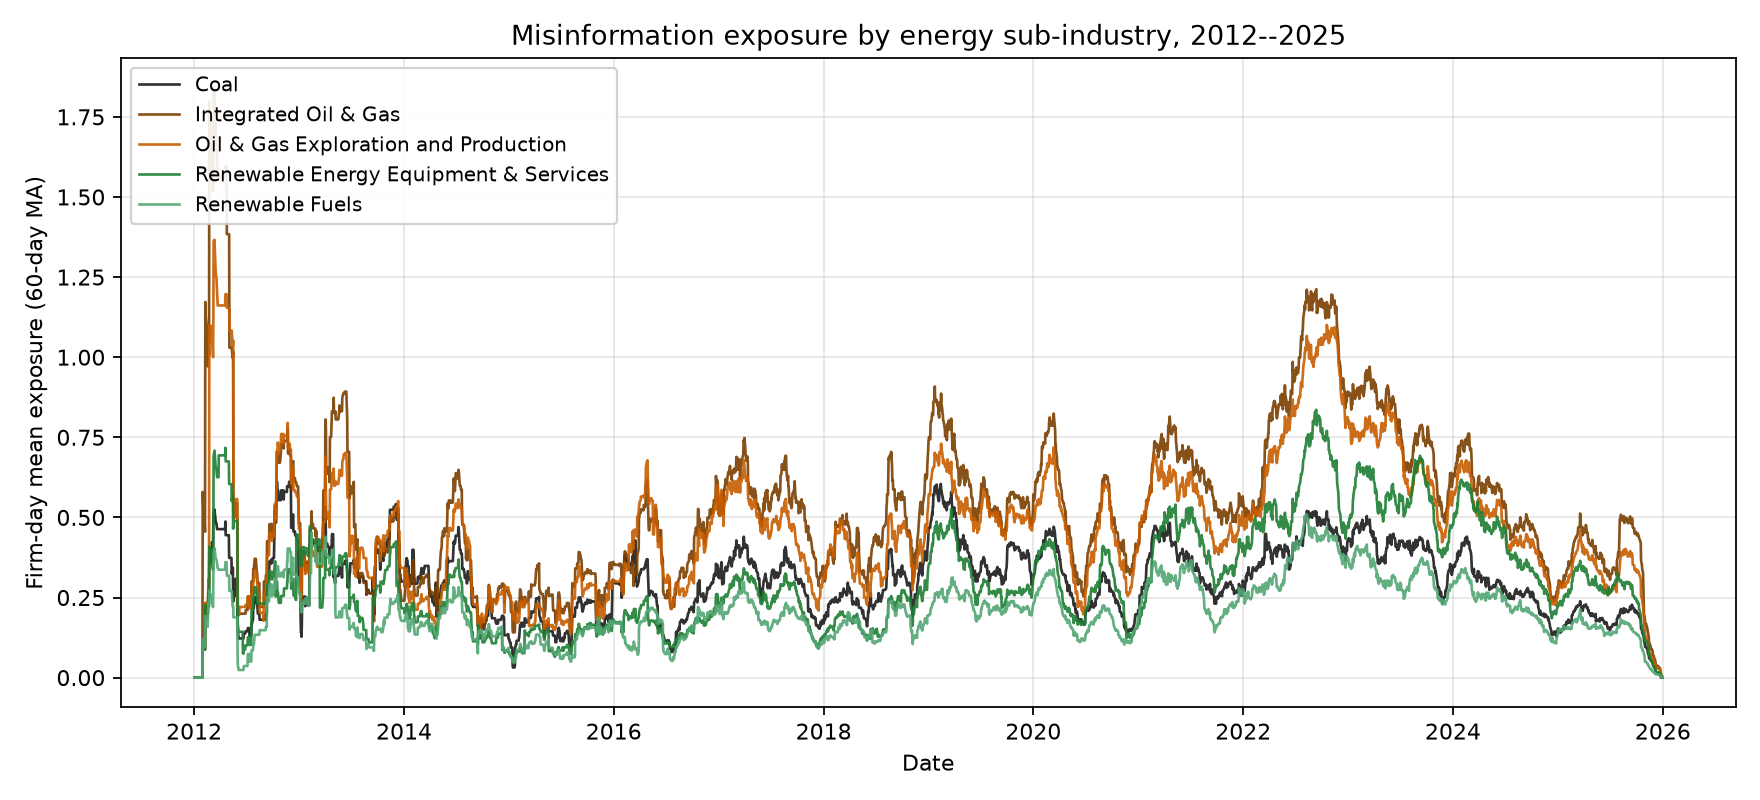
\includegraphics[width=\linewidth]{figures/fig_v2_exposure_by_industry.png}
\caption{Firm-day mean exposure by climate-transition sub-industry, 2012--2025 (60-day moving average). Fossil sub-industries trend upward after 2019; renewables are flatter. This asymmetry coincides with the post-2019 concentration of the headline spread coefficient.}
\label{fig:v2_exposure_by_industry}
\end{figure}

\subsection{Model II: Misinformation and Systematic Risk (CAPM Beta)}
\label{sec:results_modelII}

Table~\ref{tab:v2_full_modelII} reports the full readout of Equation~\ref{eq:beta_misinfo}. The CAPM beta coefficient is not distinguishable from zero in any of the headline specifications: $-0.0007$ ($p=0.53$, $N=384{,}017$) under $\mathrm{Exp}^{\text{mean}}$, $-0.0002$ ($p=0.72$) under $\log(1+\mathrm{Exp}^{\text{sum}})$, and $-0.0001$ ($p=0.21$) under $M^{\text{mean}}$. The full climate-transition panel therefore provides no statistically discernible association between day-to-day sector-specific misinformation exposure and rolling CAPM beta. The within-$R^2$ on Model II is $0.052$.

\begin{table}[htbp]
\centering
\caption{Climate-Transition Panel, PanelOLS Full Readout: Model II (CAPM Beta)}
\label{tab:v2_full_modelII}
\begin{threeparttable}
\small
\setlength{\tabcolsep}{4pt}
\begin{tabular}{l r r r r r r}
\toprule
 & \multicolumn{3}{c}{$\mathrm{Exp}^{\text{mean}}$} & \multicolumn{3}{c}{$\log(1+\mathrm{Exp}^{\text{sum}})$} \\
\cmidrule(lr){2-4}\cmidrule(lr){5-7}
Term & Coef. & SE & $p$ & Coef. & SE & $p$ \\
\midrule
Exposure term & $-0.0007$ & 0.0012 & 0.525 & $-0.0002$ & 0.0005 & 0.716 \\
Log Volume & $+0.0336^{***}$ & 0.0056 & $<$0.001 & $+0.0336^{***}$ & 0.0056 & $<$0.001 \\
Log Market Cap & $-0.0398^{**}$ & 0.0200 & 0.048 & $-0.0398^{**}$ & 0.0200 & 0.048 \\
Spread Percent & $-0.0293^{**}$ & 0.0126 & 0.021 & $-0.0293^{**}$ & 0.0126 & 0.021 \\
Dividend Yield & $-0.0074^{**}$ & 0.0036 & 0.045 & $-0.0074^{**}$ & 0.0036 & 0.045 \\
Intraday Volatility & $+0.0037^{*}$ & 0.0020 & 0.072 & $+0.0037^{*}$ & 0.0020 & 0.072 \\
CPI Inflation & $-0.0217^{***}$ & 0.0065 & 0.001 & $-0.0217^{***}$ & 0.0065 & 0.001 \\
GDP Growth & $-0.0425^{***}$ & 0.0097 & $<$0.001 & $-0.0425^{***}$ & 0.0097 & $<$0.001 \\
Unemployment & $-0.0297^{***}$ & 0.0042 & $<$0.001 & $-0.0297^{***}$ & 0.0042 & $<$0.001 \\
\midrule
Observations & & & 384,017 & & & 384,017 \\
$R^2$ & & & 0.671 & & & 0.671 \\
Within $R^2$ & & & 0.052 & & & 0.052 \\
Adj.\ Within $R^2$ & & & 0.052 & & & 0.052 \\
Wald $F$ (joint) & & & 14.26 & & & 14.26 \\
Firm FE & & & Yes & & & Yes \\
Year-Month FE & & & Yes & & & Yes \\
SE clustering & & & Firm $+$ Date & & & Firm $+$ Date \\
\bottomrule
\end{tabular}
\begin{tablenotes}
\small
\item \textit{Notes:} Dependent variable: 252-day rolling CAPM beta, Equation~\ref{eq:beta_misinfo}, 204-firm climate-transition panel. The two column blocks replace the exposure
term with the firm-day mean exposure $\mathrm{Exp}^{\text{mean}}_{i,t}$ and its
concave volume variant $\log(1+\mathrm{Exp}^{\text{sum}}_{i,t})$; control
coefficients are nearly identical across the two blocks, as expected by
Frisch--Waugh--Lovell when two variants of a sparse firm-day regressor have
negligible partial correlation with the controls. Standard errors are CRV1
two-way clustered by firm (RIC) and calendar date. Continuous controls are
winsorized at the 1st and 99th percentiles; the exposure regressors are not
winsorized. $^{*}p<0.10$, $^{**}p<0.05$, $^{***}p<0.01$.
\end{tablenotes}
\end{threeparttable}
\end{table}


The control coefficients align with standard asset-pricing intuition. Log trading volume is positively associated with beta ($+0.0336$, $p<0.001$), consistent with actively traded securities tracking aggregate market movements more closely (\cite{chordia2000commonality}; \cite{AmihudMendelson1986}). The percent quoted spread enters negatively ($-0.0293$, $p=0.021$), as expected if less liquid stocks adjust more slowly to common shocks (\cite{Hasbrouck1991}; \cite{stoll2000friction}). Dividend yield is also negative ($-0.0074$, $p=0.045$), and intraday volatility is positively associated with beta at marginal significance ($+0.0037$, $p=0.072$). Log market capitalization carries a negative coefficient ($-0.0398$, $p=0.048$), although it is subject to the same collinearity caution as the size-and-activity block in Model~I. The three macroeconomic controls all enter negatively (GDP growth $-0.0425$, unemployment $-0.0297$, CPI inflation $-0.0217$, each $p\leq 0.001$), a pattern compatible with counter-cyclical beta dynamics (\cite{StockWatson2002}; \cite{BakerBloomDavis2016}). The low within-$R^2$ reflects the construction of the 252-day rolling beta: it is a slow-moving object, most of its cross-sectional variation is absorbed by firm fixed effects, and day-level regressors explain only the marginal daily perturbation around each firm's characteristic risk profile.

The post-2019 sub-panel is the exception. The Model~II coefficient is significantly negative there ($-0.0077$, $p<0.001$; Section~\ref{sec:results_subperiod}); the same sign appears on the Japanese sub-panel ($-0.0035$, $p<0.001$). One possible explanation is short-lived decoupling from the regional market factor within the rolling estimation window rather than a durable shift in systematic risk. The size of the effect is small ($\Delta\beta \approx -0.004$ for a one-standard-deviation increase in $\mathrm{Exp}^{\text{mean}}$), and it is not present in the full-period estimate.

\subsection{Model III: Fama--French Excess Returns}
\label{sec:results_modelIII}

Table~\ref{tab:v2_full_modelIII} reports the full readout of Equation~\ref{eq:ff5_aug}. The Fama--French excess-return coefficient is negative across IV specifications and shows the largest precision gap between firm-only and two-way clustering. Under firm-only clustering on $\mathrm{Exp}^{\text{mean}}$ the coefficient is $-0.0224$ with $p<0.001$ ($N=382{,}890$); under two-way clustering the same coefficient is $-0.0224$ with $p=0.151$. The point estimate is unchanged because clustering affects the estimated standard errors rather than the coefficient; the loss of significance indicates a substantial date-level component in the residual dependence. Sector-specific misinformation exposure is associated with a small reduction in same-day excess return ($\Delta R^e \approx -0.011$ percentage points for a one-standard-deviation increase in exposure), but the association is not robust to date-level clustering and does not count as a stand-alone finding under the inference standard set in Section~\ref{sec:model}.

The log-volume and $M^{\text{mean}}$ variants of the IV produce smaller and less precise excess-return coefficients ($-0.0048$, $p=0.59$ on the log-volume; $+0.0033$, $p=0.32$ on $M^{\text{mean}}$). I therefore do not interpret Model III as carrying an independent signal in the firm-day analysis. The role of Model III in the paper is as a falsification benchmark: under H1 a daily information shock should perturb trading, not restructure return covariances, and the absence of a robust excess-return loading is consistent with that prediction even though H1's spread prediction is itself rejected.

\begin{table}[htbp]
\centering
\caption{Climate-Transition Panel, PanelOLS Full Readout: Model III (Fama--French Excess Return)}
\label{tab:v2_full_modelIII}
\begin{threeparttable}
\small
\setlength{\tabcolsep}{4pt}
\begin{tabular}{l r r r r r r}
\toprule
 & \multicolumn{3}{c}{$\mathrm{Exp}^{\text{mean}}$} & \multicolumn{3}{c}{$\log(1+\mathrm{Exp}^{\text{sum}})$} \\
\cmidrule(lr){2-4}\cmidrule(lr){5-7}
Term & Coef. & SE & $p$ & Coef. & SE & $p$ \\
\midrule
Exposure term & $-0.0224$ & 0.0156 & 0.151 & $-0.0048$ & 0.0089 & 0.591 \\
FF\_MktRF & $+0.6668^{***}$ & 0.0439 & $<$0.001 & $+0.6667^{***}$ & 0.0439 & $<$0.001 \\
FF\_SMB & $+0.2003^{***}$ & 0.0450 & $<$0.001 & $+0.2002^{***}$ & 0.0450 & $<$0.001 \\
FF\_HML & $+0.4195^{***}$ & 0.0481 & $<$0.001 & $+0.4196^{***}$ & 0.0481 & $<$0.001 \\
FF\_RMW & $+0.0066$ & 0.0345 & 0.848 & $+0.0072$ & 0.0346 & 0.835 \\
FF\_CMA & $+0.0169$ & 0.0446 & 0.704 & $+0.0171$ & 0.0446 & 0.702 \\
Log Volume & $+0.1516^{***}$ & 0.0159 & $<$0.001 & $+0.1517^{***}$ & 0.0159 & $<$0.001 \\
Log Market Cap & $+0.0677^{***}$ & 0.0215 & 0.002 & $+0.0677^{***}$ & 0.0215 & 0.002 \\
Spread Percent & $+0.1435^{***}$ & 0.0279 & $<$0.001 & $+0.1434^{***}$ & 0.0279 & $<$0.001 \\
Dividend Yield & $-0.0143^{***}$ & 0.0029 & $<$0.001 & $-0.0142^{***}$ & 0.0029 & $<$0.001 \\
Intraday Volatility & $+0.0252^{**}$ & 0.0108 & 0.021 & $+0.0252^{**}$ & 0.0108 & 0.021 \\
CPI Inflation & $+0.0008$ & 0.0119 & 0.945 & $+0.0008$ & 0.0119 & 0.946 \\
GDP Growth & $+0.0077$ & 0.0173 & 0.656 & $+0.0077$ & 0.0173 & 0.658 \\
Unemployment & $-0.0068$ & 0.0081 & 0.403 & $-0.0068$ & 0.0081 & 0.400 \\
\midrule
Observations & & & 382,890 & & & 382,890 \\
$R^2$ & & & 0.077 & & & 0.077 \\
Within $R^2$ & & & 0.069 & & & 0.069 \\
Adj.\ Within $R^2$ & & & 0.069 & & & 0.069 \\
Wald $F$ (joint) & & & 36.49 & & & 36.48 \\
Firm FE & & & Yes & & & Yes \\
Year-Month FE & & & Yes & & & Yes \\
SE clustering & & & Firm $+$ Date & & & Firm $+$ Date \\
\bottomrule
\end{tabular}
\begin{tablenotes}
\small
\item \textit{Notes:} Dependent variable: daily Fama--French five-factor excess return, Equation~\ref{eq:ff5_aug}, 204-firm climate-transition panel. The two column blocks replace the exposure
term with the firm-day mean exposure $\mathrm{Exp}^{\text{mean}}_{i,t}$ and its
concave volume variant $\log(1+\mathrm{Exp}^{\text{sum}}_{i,t})$; control
coefficients are nearly identical across the two blocks, as expected by
Frisch--Waugh--Lovell when two variants of a sparse firm-day regressor have
negligible partial correlation with the controls. Standard errors are CRV1
two-way clustered by firm (RIC) and calendar date. Continuous controls are
winsorized at the 1st and 99th percentiles; the exposure regressors are not
winsorized. $^{*}p<0.10$, $^{**}p<0.05$, $^{***}p<0.01$.
\end{tablenotes}
\end{threeparttable}
\end{table}


The factor loadings give context for the muted misinformation term. The market loading ($+0.6668$, $p<0.001$) says the average climate-transition firm captures about two-thirds of the regional daily market premium. The positive SMB loading ($+0.2003$, $p<0.001$) indicates a small-cap tilt, and the large positive HML loading ($+0.4195$, $p<0.001$) the pronounced value orientation expected of energy firms with tangible, capital-intensive assets (\cite{fama1993}; \cite{fama2015}). The profitability factor RMW ($+0.0066$, $p=0.848$) and the investment factor CMA ($+0.0169$, $p=0.704$) are both null after firm and year-month fixed effects. Among the firm-level controls, the percent quoted spread ($+0.1435$, $p<0.001$), log trading volume ($+0.1516$, $p<0.001$), log market capitalization ($+0.0677$, $p=0.002$), and intraday volatility ($+0.0252$, $p=0.021$) are positively associated with excess returns (\cite{AmihudMendelson1986}; \cite{Parkinson1980}); dividend yield is negative ($-0.0143$, $p<0.001$; \cite{FamaFrench1993}). The three macroeconomic controls are statistically indistinguishable from zero once the five factors and year-month fixed effects are included.

\section{Discussion}
\label{sec:discussion}

The strongest evidence concerns quoted spreads. Greater sector-specific misinformation exposure is associated with wider spreads ($+0.0038$, $p=0.049$; Table~\ref{tab:v2_full_modelI}), indicating lower market liquidity. The association strengthens at a one-day lag, while the sector-irrelevant placebo is statistically indistinguishable from zero. Price impact is imprecisely estimated but does not display the divergence required by liquidity fragility, so H1 is rejected. The spread pattern is instead consistent with adverse selection: when the public signal becomes less reliable, liquidity providers face greater expected losses to better-informed counterparties and widen their quotes (\cite{GlostenMilgrom1985}; \cite{EasleyOHara1992}). Climate claims about carbon restrictions, subsidies, or technology viability may be costly to verify, allowing investors with specialist knowledge to interpret their valuation implications before others. Liquidity providers may then price that informational disadvantage into quotes. This would explain why spreads widen rather than narrow: any influx of uninformed trading may be insufficient to offset the perceived risk of trading against better-informed investors. The stronger lagged association is compatible with verification and quote adjustment taking time, although the imprecise price-impact estimates and absence of direct investor-flow data prevent a definitive separation of the mechanisms.

The benchmark models qualify that interpretation without reproducing the main result. Rolling CAPM beta is essentially unchanged on the full panel (Table~\ref{tab:v2_full_modelII}), indicating that the exposure measure does not generally restructure firms' covariance with the regional market. Fama--French excess returns are negative under firm-only clustering but lose precision under two-way clustering (Table~\ref{tab:v2_full_modelIII}), so Model~III does not support an independent return effect. The strongest evidence therefore concerns trading costs rather than systematic risk or return premia.

The political-economy implication is most direct at the sub-industry level. The evidence emerges once the regressor varies within a day across the nine TRBC energy sub-industries---fossil chains versus renewables, integrated production versus refining, and coal versus oil services. A coal-firm trader on a high-exposure day faces a different information environment from a renewable-fuels trader on the same day. A market-wide daily index cannot represent that distinction, which is central to identifying the spread association.

Two checks bear on the climate-specific interpretation. First, when the firm-day index is rebuilt from only those posts the same model judges sector-irrelevant ($R_{p,s}<10$), the Model~I coefficient is statistically indistinguishable from zero ($-0.018$, $p=0.35$). The null placebo does not reproduce the headline positive spread association, supporting---but not establishing---the sector-specific interpretation. Second, the positive spread association is statistically discernible in 2019--2025, alongside greater corpus volume and a wider fossil--renewable exposure gap (Figure~\ref{fig:v2_exposure_by_industry}). Those changes may affect measurement precision and sample composition; they do not establish that the underlying relationship is stronger in that period. The subperiod estimates require a formal coefficient-difference test before they can be interpreted as evidence of a change in the relationship.

The reach-based channel emphasized by \textcite{acemoglu2010spread} and \textcite{VosoughiRoyAral2018} has a natural interpretation in the present design. The log-volume variant of the regressor---which is sensitive to the number of sector-relevant climate posts a firm's sub-industry sees on a given day---has the most precisely estimated Model~I coefficient ($p=0.001$). This pattern may be compositional rather than purely volume-driven because high-volume climate-post days are also high-engagement days. The data do not separate volume from engagement empirically because the classification was performed without engagement weights; doing so would require comparing an engagement-weighted firm-day index with the unweighted measure. The current evidence is consistent with a compositional reading but does not identify it.

For the political economy of climate finance, two implications follow. First, the association between sector-specific climate misinformation and trading costs runs in the direction adverse-selection theory predicts---wider, not narrower, quoted spreads---and is concentrated after 2019, when corpus volume and sub-industry differentiation increase. The regional estimates are directionally suggestive but imprecise. Second, measurement matters as much as model choice. Future work should construct firm-day regressors at the level at which political content varies rather than aggregate across firms whose substantive exposure differs.

\section{Conclusions}
\label{sec:conclusion}

The results for climate-transition firms show a clear pattern. Firms with greater exposure to climate misinformation have significantly wider quoted bid--ask spreads, indicating lower market liquidity. This relationship remains statistically significant after accounting for firm and time effects and becomes stronger one day after exposure, suggesting that the market's response is not immediate but strengthens over time. Price impact does not move in the opposite direction, so the divergence between the two liquidity measures required by H1 is absent. The evidence rejects the liquidity-fragility prediction and is more consistent with adverse-selection pressure.

Four conclusions follow. First, evidence that discriminates between H1 and the adverse-selection alternative becomes visible only once the misinformation regressor is constructed with cross-sectional variation across firms within a calendar day. A market-wide daily index of misinformation diffusion, applied to the same panel of climate-transition firms, returns the opposite sign with no statistical significance, and the two regressors are nearly orthogonal ($r=0.10$). The political-economy content of climate misinformation is partitioned along the sub-industry axis, not along the calendar-day axis, and the association is most clearly identified when the regressor respects that partition.

Second, the rolling CAPM beta response is small and not robust on the full climate-transition panel. This is consistent with a change in the day's trading environment rather than a restructuring of rolling return covariances. The exception is the post-2019 sub-panel, where the beta loading is significantly negative; given its small magnitude and absence in the full panel, I do not interpret it as a structural shift in systematic risk.

Third, the Fama--French excess-return response is negative under firm-only clustering but loses precision under two-way clustering. Model~III is therefore not a stand-alone finding. The pattern is consistent with H1's benchmark expectation that a daily information shock should perturb trading rather than restructure return premia, but the present data do not support a robust excess-return interpretation.

Fourth, the post-2019 concentration of the headline spread coefficient is the most pronounced temporal pattern in the analysis. Before 2019 the regressor is not associated with any outcome; after 2019 it is associated with wider spreads and a negative beta coefficient, while the excess-return estimate remains imprecise. The contemporaneous increase in corpus volume and fossil--renewable exposure differences (Figure~\ref{fig:v2_exposure_by_industry}) may change measurement precision and composition, but does not establish a stronger underlying relationship after 2019. The empirical claim is therefore conditional: during 2019--2025, exposure to climate misinformation in the English-language Facebook corpus is associated with trading costs in the direction adverse-selection theory predicts.

For the political economy of climate finance, the daily contest over climate information is reflected in wider quoted spreads among firms whose sub-industries are the subject of the contested content. The estimated magnitude is modest ($\sim$1.2\% of the unconditional mean spread for a one-standard-deviation increase in exposure) and is concentrated in the post-2019 period. Classifying misinformation at the sub-industry level preserves cross-sectional variation that a market-wide daily index loses. Future work can move in three directions. An instrumental-variable or event-study design built on exogenous political triggers---a court ruling, a leaked memo, a viral hoax---is needed to move from association to identification. Direct retail-flow data would help distinguish adverse selection from a residual attention channel. The firm-day exposure construction could also be applied to other domains of politically contested knowledge---public health, technology regulation, and financial regulation---to test whether the pattern extends beyond climate (\cite{lins2017social}; \cite{taber2006motivated}).

\printbibliography

\appendix
\section*{Appendix} 
Section~\ref{sec:appendix_financial} reports descriptive statistics for the financial panel (Tables~\ref{tab:panel_a}--\ref{tab:panel_f}), and Section~\ref{sec:appendix_climate} reports coverage and composition for the climate-transition equity panel. Section~\ref{sec:appendix_corpus} documents the misinformation corpus (Tables~\ref{tab:panel_g}--\ref{tab:panel_n}), including misinformation type and reach in Section~\ref{sec:firmday_corpus_intuition}. Section~\ref{sec:appendix_network} maps the dissemination network, Section~\ref{sec:firmday_validation} describes and validates the firm-day exposure index, and Section~\ref{sec:appendix_heterogeneity} reports the heterogeneity and interaction checks.

\section{Financial Panel Descriptive Statistics}
\label{sec:appendix_financial}

The merged firm-level panel comprises 19,183,738 firm-day observations across 5,375 unique equity securities spanning 2012--2025. Table~\ref{tab:panel_a} reports summary statistics - including observation counts, fill rates, means, standard deviations, and full distributional percentiles - for nine firm-level trading variables (prices, volume, market capitalization, dividend yield, bid-ask spreads, returns, and CAPM beta), three macroeconomic controls (GDP growth, unemployment, CPI inflation), and the five Fama-French factors (MktRF, SMB, HML, RMW, CMA). The table is presented in landscape orientation to accommodate the eleven-column layout.

\begin{sidewaystable}[htbp]
\centering
\footnotesize
\setlength{\tabcolsep}{3.5pt}
\begin{tabular}{l l r r r r r r r r r}
\toprule
\textbf{Variable} & \textbf{Unit} & \textbf{N} & \textbf{Fill\%} & \textbf{Mean} & \textbf{SD} & \textbf{Min} & \textbf{P25} & \textbf{Median} & \textbf{P75} & \textbf{Max} \\
\midrule
\multicolumn{11}{l}{\textit{Firm-Level Variables}} \\
  Price Close & USD & 13,759,934 & 71.7 & 388.67 & 2,128.98 & 0.01 & 10.96 & 30.58 & 118.26 & 359,900.00 \\
  Volume & shares & 18,394,237 & 95.9 & 9.03M & 60.58M & 0.00 & 0.00 & 0.823M & 5.08M & 45,941.76M \\
  Company Market Cap & USD (thousands) & 14,263,811 & 74.4 & 1,860,901.54 & 21,101,237.64 & 14.87 & 5,032.21 & 15,080.74 & 104,672.42 & 2,464,175,093.59 \\
  Dividend yield & \% & 12,626,836 & 65.8 & 2.38 & 8.49 & 0.00 & 0.48 & 1.72 & 3.49 & 20,316.87 \\
  BidAskSpread & USD & 13,419,146 & 70.0 & 4.24 & 61.02 & -268.00 & 0.01 & 0.04 & 0.30 & 13,550.00 \\
  SpreadPercent & \% & 13,419,145 & 70.0 & 0.54 & 1.95 & -200.00 & 0.07 & 0.16 & 0.37 & 172.14 \\
  DailyReturn &  & 13,255,243 & 69.1 & 0.09 & 115.33 & -73.29 & -1.04 & 0.00 & 1.01 & 419,653.09 \\
  CAPM\_Beta &  & 13,802,427 & 71.9 & 0.54 & 0.48 & -11.74 & 0.22 & 0.47 & 0.82 & 298.91 \\
  TotalReturn &  & 13,735,222 & 71.6 & 0.10 & 113.30 & -98.58 & -1.04 & 0.00 & 1.02 & 419,653.09 \\
\midrule
\multicolumn{11}{l}{\textit{Macroeconomic Controls}} \\
  GDP Growth & \% & 19,183,738 & 100.0 & 3.55 & 2.90 & -10.05 & 1.82 & 2.79 & 6.07 & 8.57 \\
  Unemployment & \% & 19,183,738 & 100.0 & 74.87 & 12.97 & 53.10 & 63.52 & 80.07 & 82.02 & 92.19 \\
  CPI Inflation & \% & 19,183,738 & 100.0 & 1.89 & 1.52 & -0.23 & 0.98 & 1.92 & 2.62 & 8.83 \\
\midrule
\multicolumn{11}{l}{\textit{Fama--French Five Factors}} \\
  FF MktRF & \% & 18,987,538 & 99.0 & 0.03 & 1.01 & -12.01 & -0.44 & 0.05 & 0.55 & 10.03 \\
  FF SMB & \% & 18,987,538 & 99.0 & -0.01 & 0.53 & -4.81 & -0.30 & 0.00 & 0.29 & 5.71 \\
  FF HML & \% & 18,987,538 & 99.0 & 0.01 & 0.66 & -5.03 & -0.32 & 0.00 & 0.33 & 6.73 \\
  FF RMW & \% & 18,987,538 & 99.0 & 0.01 & 0.43 & -3.76 & -0.23 & 0.00 & 0.25 & 4.25 \\
  FF CMA & \% & 18,987,538 & 99.0 & 0.00 & 0.40 & -2.92 & -0.21 & 0.00 & 0.21 & 2.47 \\
\bottomrule
\end{tabular}
\caption{Panel~A: Summary statistics for key variables in the merged dataset. The sample spans 2012--2025 and covers 5,375 RICs. Fill\% indicates the proportion of non-missing observations for each variable. All firm-level variables are at daily frequency.}
\label{tab:panel_a}
\end{sidewaystable}

The equity universe spans five geographic regions with heterogeneous market structures and data availability. Table~\ref{tab:panel_b} reports the number of firm-day observations and unique RICs per region, alongside fill rates for closing prices, CAPM beta, and Fama-French factors. China contributes the largest share of observations (41.2\%), followed by the United States (31.7\%) and Japan (23.8\%), while the UK and EU together account for approximately 3.4\% of the sample.

\begin{table}[!ht]
\centering
\footnotesize
\begin{tabular}{l r r r r r r r r}
\toprule
\textbf{Region} & \textbf{Obs} & \textbf{Share\%} & \textbf{RICs} & \textbf{First} & \textbf{Last} & \textbf{Price\%} & \textbf{Beta\%} & \textbf{FF\%} \\
\midrule
  CN & 7,897,640 & 41.2 & 2,231 & 2012-01-02 & 2025-12-31 & 62.3 & 63.0 & 100.0 \\
  US & 6,075,274 & 31.7 & 1,712 & 2012-01-02 & 2025-12-31 & 71.6 & 69.7 & 97.0 \\
  JP & 4,558,053 & 23.8 & 1,253 & 2012-01-02 & 2025-12-31 & 85.2 & 87.4 & 99.7 \\
  UK & 364,446 & 1.9 & 100 & 2012-01-02 & 2025-12-31 & 93.4 & 92.7 & 100.0 \\
  EU & 288,325 & 1.5 & 79 & 2012-01-02 & 2025-12-31 & 94.2 & 92.8 & 100.0 \\
\midrule
  \textbf{Total} & \textbf{19,183,738} & 100.0 & \textbf{5,375} & & & & & \\
\bottomrule
\end{tabular}
\caption{Panel~B: Coverage by region. Share\% is the fraction of total firm-day observations. Price\%, Beta\%, and FF\% indicate the fill rate for Price Close, CAPM Beta, and Fama--French factors, respectively.}
\label{tab:panel_b}
\end{table}

Temporal stability is a desirable property for panel econometric analysis, as changing panel composition can introduce survivorship bias. Table~\ref{tab:panel_c} reports annual observation counts, the number of distinct securities, and non-missing rates for key variables across all fourteen sample years. The constant RIC count of 5,375 per year confirms a balanced panel structure, while data fill rates for prices, returns, and betas increase monotonically over time as coverage improves.

\begin{table}[!ht]
\centering
\footnotesize
\begin{tabular}{r r r r r r}
\toprule
\textbf{Year} & \textbf{Obs} & \textbf{RICs} & \textbf{Price\%} & \textbf{Return\%} & \textbf{Beta\%} \\
\midrule
  2012 & 1,363,092 & 5,375 & 53.6 & 51.3 & 25.2 \\
  2013 & 1,356,566 & 5,375 & 54.7 & 52.2 & 57.3 \\
  2014 & 1,366,584 & 5,375 & 55.8 & 53.3 & 58.0 \\
  2015 & 1,365,143 & 5,375 & 56.9 & 54.4 & 59.4 \\
  2016 & 1,367,945 & 5,375 & 59.3 & 56.5 & 61.2 \\
  2017 & 1,360,941 & 5,375 & 64.4 & 61.8 & 64.9 \\
  2018 & 1,368,416 & 5,375 & 68.1 & 65.4 & 70.3 \\
  2019 & 1,373,060 & 5,375 & 71.3 & 68.5 & 73.4 \\
  2020 & 1,376,595 & 5,375 & 75.4 & 72.7 & 76.8 \\
  2021 & 1,377,392 & 5,375 & 82.4 & 80.0 & 83.1 \\
  2022 & 1,373,896 & 5,375 & 87.2 & 84.6 & 89.3 \\
  2023 & 1,372,026 & 5,375 & 90.1 & 87.4 & 93.1 \\
  2024 & 1,382,316 & 5,375 & 91.8 & 88.8 & 96.5 \\
  2025 & 1,379,766 & 5,375 & 92.4 & 89.6 & 97.7 \\
\bottomrule
\end{tabular}
\caption{Panel~C: Annual coverage. Obs is the number of firm-day observations per year; RICs is the number of distinct securities observed that year. Price\%, Return\%, and Beta\% are non-missing rates for Price Close, DailyReturn, and CAPM Beta.}
\label{tab:panel_c}
\end{table}

Before estimating the main regression specifications, it is useful to examine the bivariate relationships among key continuous variables for evidence of multicollinearity or unexpected sign patterns. Table~\ref{tab:panel_d} presents the upper-triangle pairwise correlation matrix for daily returns, CAPM beta, percentage bid--ask spread, volume, market capitalization, and the three primary Fama-French factors. Correlations are generally modest in magnitude, with the largest off-diagonal entries appearing between MktRF and SMB ($r = -0.14$) and between MktRF and HML ($r = -0.15$).

\begin{table}[!ht]
\centering
\footnotesize
\setlength{\tabcolsep}{4pt}
\begin{tabular}{lrrrrrrrr}
\toprule
 & \textbf{Return} & \textbf{Beta} & \textbf{Spread\%} & \textbf{Volume} & \textbf{MktCap} & \textbf{MktRF} & \textbf{SMB} & \textbf{HML} \\
\midrule
  Return & 1.00 & 0.17 & 0.02 & 0.00 & 0.03 & 0.00 & -0.00 & -0.00 \\
  Beta &  & 1.00 & -0.23 & -0.01 & -0.05 & -0.00 & -0.00 & -0.00 \\
  Spread\% &  &  & 1.00 & -0.02 & 0.01 & 0.00 & -0.00 & -0.01 \\
  Volume &  &  &  & 1.00 & 0.07 & -0.00 & 0.00 & 0.00 \\
  MktCap &  &  &  &  & 1.00 & 0.00 & -0.00 & -0.00 \\
  MktRF &  &  &  &  &  & 1.00 & -0.14 & -0.15 \\
  SMB &  &  &  &  &  &  & 1.00 & 0.05 \\
  HML &  &  &  &  &  &  &  & 1.00 \\
\bottomrule
\end{tabular}
\caption{Panel~D: Pairwise correlations among key variables. Empty cells below the diagonal are suppressed for readability.}
\label{tab:panel_d}
\end{table}

Fama-French factor returns are matched to each firm based on its listing region, with four regional factor sets covering Asia Pacific, the United States, Japan, and Europe. Table~\ref{tab:panel_e} reports the number of matched observations, fill rates, and mean daily values for all five factors by region. The US market excess return exhibits the highest mean (0.056\% per day), while Japan exhibits the largest standard deviation (1.153\%).

\begin{table}[!ht]
\centering
\footnotesize
\begin{tabular}{l r r r r r r r r}
\toprule
\textbf{FF Region} & \textbf{Obs} & \textbf{Fill\%} & \textbf{MktRF} & \textbf{SD(MktRF)} & \textbf{SMB} & \textbf{HML} & \textbf{RMW} & \textbf{CMA} \\
\midrule
  AsiaPac & 7,897,640 & 100.0 & 0.019 & 0.856 & -0.007 & 0.021 & 0.018 & 0.006 \\
  US & 6,075,274 & 97.0 & 0.056 & 1.084 & -0.009 & -0.003 & 0.006 & -0.003 \\
  Japan & 4,558,053 & 99.7 & 0.033 & 1.153 & 0.002 & 0.012 & 0.000 & 0.005 \\
  Europe & 652,771 & 100.0 & 0.033 & 1.028 & 0.000 & 0.009 & 0.006 & 0.001 \\
\bottomrule
\end{tabular}
\caption{Panel~E: Fama-French five-factor summary by region mapping. Mean daily factor returns are reported. Fill\% indicates the proportion of firm-day observations matched to factors.}
\label{tab:panel_e}
\end{table}

The microstructure variables reported in Table~\ref{tab:panel_f} include the percent quoted spread and per-dollar price impact used as the primary and companion liquidity outcomes. The table documents observation counts, the number of securities with non-missing data, and distributional summaries for eight trade-level variables: bid--ask spread, percentage spread, order flow, trade intensity, buyer- and seller-initiated trade indicators, volume-weighted average price (VWAP), and price impact. Coverage is near-universal for spread and order-flow variables (5,343 of 5,375 RICs) but lower for trade intensity (2,029 RICs), reflecting cross-exchange differences in tick-level data availability.

\begin{table}[!ht]
\centering
\footnotesize
\begin{tabular}{l r r r r r}
\toprule
\textbf{Variable} & \textbf{N} & \textbf{RICs} & \textbf{Mean} & \textbf{SD} & \textbf{Median} \\
\midrule
  BidAskSpread & 13,419,146 & 5,343 & 4.24 & 61.02 & 0.04 \\
  SpreadPercent & 13,419,145 & 5,343 & 0.54 & 1.95 & 0.16 \\
  OrderFlow & 13,268,923 & 5,343 & 0.08 & 193.08 & 0.00 \\
  TradeIntensity & 5,146,749 & 2,029 & 4,750.04 & 12,478.89 & 2,198.00 \\
  BuyerInitiated & 13,837,387 & 5,343 & 0.48 & 0.50 & 0.00 \\
  SellerInitiated & 13,837,387 & 5,343 & 0.47 & 0.50 & 0.00 \\
  VWAP & 13,584,674 & 5,343 & 392.92 & 2,115.66 & 30.53 \\
  PriceImpact & 13,268,922 & 5,343 & 0.68 & 47.95 & 0.37 \\
\bottomrule
\end{tabular}
\caption{Panel~F: Microstructure-variable coverage. The percent quoted spread and price impact are the liquidity outcomes used in the main analysis. N is the number of non-missing observations; RICs is the number of distinct securities with at least one non-missing value.}
\label{tab:panel_f}
\end{table}

\begin{table}[htbp]
\centering
\caption{Mean CAPM Beta by Region and Market-Capitalisation Quintile}
\label{tab:beta_region_mktcap}
\begin{threeparttable}
\small
\begin{tabular}{l r r r r r r}
\toprule
Region & Mean $\beta$ & Median $\beta$ & Q1 (Small) & Q2 & Q3 & Q5 (Large) \\
\midrule
CN & 0.655 & 0.594 & 0.643 & 0.673 & 0.667 & 0.600 \\
US & 0.488 & 0.388 & 0.806 & 0.837 & 0.823 & 0.166 \\
JP & 0.415 & 0.330 & 0.263 & 0.283 & 0.303 & 0.825 \\
UK & 0.747 & 0.714 & 0.731 & 0.785 & 0.782 & 0.570 \\
EU & 0.905 & 0.877 & 0.816 & 0.967 & 0.897 & 0.995 \\
\bottomrule
\end{tabular}
\begin{tablenotes}\small
\item \textit{Notes:} Mean rolling CAPM beta computed from 252-day OLS windows requiring minimum 126 observations. Quintiles defined by Company Market Cap within each region-day. The low overall mean (0.54) is driven by Japanese firms (0.42) and the preponderance of small-cap US firms in the sample. Non-synchronous trading bias (\cite{ScholesWilliams1977}) likely contributes to downward bias in thinly traded securities.
\end{tablenotes}
\end{threeparttable}
\end{table}

\FloatBarrier
\section{Climate-Transition Panel Descriptive Statistics}
\label{sec:appendix_climate}

This subsection reports descriptive statistics for the unique climate-transition firm panel used in the subsample regressions. The objective is to document coverage, composition, and distributional properties before estimation. Across all three tables below, the sample is defined by renewable and fossil-fuel TRBC mappings with utilities excluded, consistent with the main-text climate-transition specifications.

\begin{table}[htbp]
\centering
\caption{Climate-Transition Panel Coverage Summary}
\label{tab:energy_desc_coverage}
\begin{threeparttable}
\small
\begin{tabular}{l r}
\toprule
Metric & Value \\
\midrule
Firm-day observations & 726,890 \\
Unique firms (RICs) & 204 \\
Start date & 2012-01-02 \\
End date & 2025-12-31 \\
Unique year-month bins & 168 \\
Median observations per firm & 3,588 \\
\bottomrule
\end{tabular}
\begin{tablenotes}\small
\item \textit{Notes:} Coverage statistics for the climate-transition panel used in the fixed-effects regressions.
\end{tablenotes}
\end{threeparttable}
\end{table}

\begin{table}[htbp]
\centering
\caption{Climate-Transition Panel Composition by Region (Unique Firms)}
\label{tab:energy_desc_region}
\begin{threeparttable}
\small
\begin{tabular}{l r r}
\toprule
Region & Unique firms & Share (\%) \\
\midrule
US & 102 & 50.00 \\
CN & 83 & 40.69 \\
JP & 15 & 7.35 \\
EU & 2 & 0.98 \\
UK & 2 & 0.98 \\
\bottomrule
\end{tabular}
\begin{tablenotes}\small
\item \textit{Notes:} Shares are calculated over the 204 unique firms in the climate-transition sample.
\end{tablenotes}
\end{threeparttable}
\end{table}

\begin{table}[htbp]
\centering
\caption{Climate-Transition Panel Key Variable Descriptive Statistics}
\label{tab:energy_desc_vars}
\begin{threeparttable}
\small
\setlength{\tabcolsep}{4pt}
\begin{tabular}{l r r r r r r}
\toprule
Variable & N & Mean & Std. Dev. & P25 & Median & P75 \\
\midrule
SpreadPercent & 504,043 & 0.6147 & 1.6705 & 0.0607 & 0.1590 & 0.4090 \\
CAPM\_Beta & 525,697 & 0.5679 & 0.4984 & 0.2039 & 0.5168 & 0.8864 \\
ExcessReturn & 506,612 & 0.0328 & 2.6949 & -1.2207 & -0.0100 & 1.1272 \\
log\_volume & 698,179 & 11.3694 & 6.8472 & 5.7071 & 14.5147 & 16.3631 \\
log\_mktcap & 559,387 & 25.0607 & 2.7631 & 22.9046 & 24.3402 & 27.1216 \\
IntradayVolatility & 496,614 & 3.4611 & 2.5748 & 1.7758 & 2.7528 & 4.3222 \\
DivYield & 464,457 & 2.9153 & 3.6049 & 0.2509 & 1.8536 & 4.1325 \\
cpi\_inflation & 726,890 & 2.1371 & 1.5976 & 1.2616 & 2.0000 & 2.6195 \\
gdp\_growth & 726,890 & 3.8414 & 2.6520 & 2.3402 & 2.8876 & 6.0685 \\
unemployment & 726,890 & 73.1123 & 11.1097 & 63.5234 & 80.0325 & 80.4977 \\
\bottomrule
\end{tabular}
\begin{tablenotes}\small
\item \textit{Notes:} Statistics correspond to the estimation sample after standard preprocessing used in the econometric pipeline (including transformations and winsorisation for relevant continuous variables).
\end{tablenotes}
\end{threeparttable}
\end{table}

The descriptive profile in Tables~\ref{tab:energy_desc_coverage}--\ref{tab:energy_desc_vars} motivates the energy-subsample strategy. The panel is sufficiently long and dense for two-way FE estimation, yet composition is concentrated in US and Chinese firms, making firm-level fixed effects and clustered inference essential.

\FloatBarrier
\FloatBarrier
\section{Descriptive Statistics and Supporting Tables}
\label{sec:appendix_corpus}

The corpus comprises 265,652 public Facebook posts with platform-reported engagement data. Table~\ref{tab:panel_g} provides distributional summaries for all engagement metrics - likes, shares, comments, total reactions (including emoji-specific breakdowns for angry, love, haha, sad, wow, and care reactions), and view counts - as well as text-level characteristics (character length and word count). The large gap between mean and median values for most engagement variables reflects the heavy right skew characteristic of social media diffusion, where a small number of viral posts account for a disproportionate share of total engagement.

\begin{table}[!ht]
\centering
\caption{Social Media Post Summary Statistics}
\label{tab:panel_g}
\begin{threeparttable}
\begin{tabularx}{\textwidth}{l R R R R R R}
\toprule
Variable & N & Mean & Median & Std.Dev. & Min & Max \\
\midrule
Likes & 262,461 & 140.8 & 10.00 & 2,015.6 & 0.000 & 525,472.0 \\
Shares & 265,651 & 44.90 & 2.00 & 682.3 & 0.000 & 81,948.0 \\
Comments & 265,651 & 22.72 & 0.000 & 217.6 & 0.000 & 39,790.0 \\
Total Reactions & 262,492 & 175.9 & 13.00 & 2,278.2 & 0.000 & 531,508.0 \\
Views & 220,511 & 10,372.8 & 1,625.0 & 91,127.8 & 101.0 & 15,900,642 \\
Angry Reactions & 262,461 & 7.69 & 0.000 & 225.5 & 0.000 & 57,470.0 \\
Love Reactions & 262,461 & 15.38 & 0.000 & 267.5 & 0.000 & 46,490.0 \\
Haha Reactions & 262,461 & 3.84 & 0.000 & 89.18 & 0.000 & 31,575.0 \\
Sad Reactions & 262,461 & 3.52 & 0.000 & 162.2 & 0.000 & 44,420.0 \\
Wow Reactions & 262,461 & 1.66 & 0.000 & 31.79 & 0.000 & 7,074.0 \\
Care Reactions & 262,461 & 0.000 & 0.000 & 0.000 & 0.000 & 0.000 \\
Text Length (chars) & 265,652 & 3,599.1 & 1,337.0 & 6,828.6 & 2.00 & 168,477.0 \\
Word Count & 265,652 & 553.9 & 197.0 & 1,062.6 & 1.00 & 26,148.0 \\
\bottomrule
\end{tabularx}
\begin{tablenotes}\small
\item \textit{Notes:} Summary statistics for 265,652 social media posts from the Meta Content Library (MCL). Engagement metrics reflect platform-reported counts at the time of data collection.
\end{tablenotes}
\end{threeparttable}
\end{table}

The 217,954 unique posts paired by calendar date to the climate-transition panel span 2012 through 2025. Table~\ref{tab:panel_j} reports their annual distribution, with the misinformation classification produced by the Qwen3.6-35B-A3B model (Section~\ref{sec:LLM}): a post is counted as misinformation if its continuous misinformation score reaches the rubric's ``clearly false or pseudoscientific climate/energy claims'' threshold of 50 on the 0--100 scale. Post volume rises sharply after 2019, coinciding with the intensification of global climate activism and the digital migration associated with the COVID-19 pandemic, while Qwen-classified misinformation prevalence fluctuates between 1.7\% and 5.0\% across years. The within-year movement reflects climate-political intensity rather than raw volume: prevalence peaks in the contested-policy years 2012 (5.0\%), 2017 (3.0\%), 2019 (3.2\%), and 2022 (3.0\%), and falls to its sample minimum in the highest-volume years 2024--2025 ($\approx$1.7\%), where general climate content grows faster than misinformation.

\begin{table}[!ht]
\centering
\caption{Annual Distribution of Posts and Qwen-Classified Misinformation Prevalence}
\label{tab:panel_j}
\begin{threeparttable}
\begin{tabularx}{\textwidth}{l R R R R R}
\toprule
Year & Total Posts & Misinfo.\ Posts & Prevalence (\%) & Mean Likes & Mean Shares \\
\midrule
2012 & 1,276 & 64 & 5.02 & 86.2 & 38.96 \\
2013 & 2,649 & 82 & 3.10 & 87.5 & 39.97 \\
2014 & 3,885 & 88 & 2.27 & 87.8 & 33.56 \\
2015 & 5,106 & 95 & 1.86 & 115.5 & 47.93 \\
2016 & 9,954 & 272 & 2.73 & 138.2 & 82.97 \\
2017 & 13,845 & 413 & 2.98 & 93.7 & 58.13 \\
2018 & 11,429 & 268 & 2.34 & 66.2 & 45.01 \\
2019 & 17,160 & 542 & 3.16 & 90.6 & 47.83 \\
2020 & 17,118 & 427 & 2.49 & 128.0 & 61.19 \\
2021 & 23,038 & 469 & 2.04 & 112.9 & 38.67 \\
2022 & 24,102 & 710 & 2.95 & 86.9 & 22.68 \\
2023 & 25,846 & 731 & 2.83 & 76.7 & 21.54 \\
2024 & 30,404 & 538 & 1.77 & 88.3 & 26.95 \\
2025 & 32,142 & 552 & 1.72 & 344.6 & 62.91 \\
\midrule
Total & 217,954 & 5,251 & 2.41 & 132.4 & 43.03 \\
\bottomrule
\end{tabularx}
\begin{tablenotes}\small
\item \textit{Notes:} Annual counts for the 217,954 unique posts paired by date to the climate-transition panel. ``Misinfo.\ Posts'' counts posts whose Qwen3.6-35B-A3B misinformation score reaches the threshold of 50; ``Prevalence'' is that count as a share of the year's posts.
\end{tablenotes}
\end{threeparttable}
\end{table}

The Meta Content Library organizes posts into eight keyword-based thematic datasets covering different dimensions of climate discourse. Table~\ref{tab:panel_k} breaks down post coverage, Qwen-classified misinformation counts, engagement, and unique owner counts by source dataset. The pattern is intuitive given how the model reasons about content: the explicitly political ``combined'' multi-keyword set (6.4\% prevalence) and the climate-politics set (1.9\%) concentrate the misinformation, because that is where contested claims about climate science and policy are made, whereas the adaptation, resilience, and ecological datasets---which collect operational and scientific content---sit at or below 0.2\% prevalence. The classifier is not flagging climate \emph{topicality}; it is flagging the false or misleading \emph{claims} that cluster in the political corners of the corpus.

\begin{table}[!ht]
\centering
\caption{Post Coverage by MCL Source Dataset (Qwen-Classified Misinformation)}
\label{tab:panel_k}
\begin{threeparttable}
\begin{tabularx}{\textwidth}{l R R R R R R}
\toprule
Source Dataset & Posts & Misinfo. & Prev.\ (\%) & Mean Likes & Mean Shares & Owners \\
\midrule
Combined & 65,688 & 4,180 & 6.4 & 144.8 & 69.73 & 25,171 \\
Climate Change Adaptation Al.. & 61,079 & 126 & 0.2 & 48.10 & 11.12 & 17,931 \\
Climate Change Politics All .. & 32,930 & 618 & 1.9 & 153.2 & 69.05 & 14,527 \\
Climate Change Global Justic.. & 14,406 & 134 & 0.9 & 120.4 & 38.57 & 7,369 \\
Climate Change Global Resili.. & 13,448 & 18 & 0.1 & 68.60 & 11.55 & 7,019 \\
Climate Change Activism All .. & 11,222 & 149 & 1.3 & 639.8 & 62.98 & 6,120 \\
Ecological Resilience All Time & 9,835 & 8 & 0.1 & 77.90 & 16.27 & 5,710 \\
Ecological Justice All Time & 9,346 & 18 & 0.2 & 77.30 & 28.76 & 4,984 \\
\bottomrule
\end{tabularx}
\begin{tablenotes}\small
\item \textit{Notes:} The 217,954 paired posts drawn from eight MCL keyword-based search datasets. ``Combined'' denotes the multi-keyword merged set. ``Misinfo.''\ counts posts with Qwen3.6-35B-A3B misinformation score $\geq 50$; ``Owners'' is the count of distinct posting accounts per dataset.
\end{tablenotes}
\end{threeparttable}
\end{table}

Understanding who produces misinformation requires examining the distribution of posting activity across the 55,699 unique post owners in the paired corpus. Table~\ref{tab:panel_l} groups owners into five activity brackets and reports each bracket's contribution to total volume and Qwen-classified misinformation output. The distribution is heavily right-skewed: over half of all owners contribute only a single post, while 124 heavy posters (more than 100 posts each) account for roughly 12\% of total volume. The Qwen misinformation rate is broadly stable across brackets (1.3\%--2.6\%), which carries a substantive point---misinformation in this corpus is not the product of a small set of hyperactive accounts but is distributed across the full activity range, including the long tail of one-time posters. The dissemination problem is therefore one of breadth rather than concentration in supply, even if reach (Section~\ref{sec:firmday_corpus_intuition}) is far more skewed than production.

\begin{table}[!ht]
\centering
\caption{Post Owner Activity and Qwen-Classified Misinformation Concentration}
\label{tab:panel_l}
\begin{threeparttable}
\begin{tabularx}{\textwidth}{l R R R R R}
\toprule
Activity Bracket & Owners & Total Posts & \% of Corpus & Misinfo.\ Posts & Misinfo.\ Rate (\%) \\
\midrule
1 post & 30,528 & 30,528 & 14.0 & 669 & 2.19 \\
2--10 posts & 21,627 & 78,690 & 36.1 & 2,000 & 2.54 \\
11--50 posts & 3,152 & 63,464 & 29.1 & 1,639 & 2.58 \\
51--100 posts & 268 & 18,280 & 8.4 & 233 & 1.27 \\
$>$100 posts & 124 & 26,990 & 12.4 & 710 & 2.63 \\
\midrule
Total & 55,699 & 217,952 & 100.0 & 5,251 & 2.41 \\
\bottomrule
\end{tabularx}
\begin{tablenotes}\small
\item \textit{Notes:} Owners of the 217,954 paired posts (two posts have no owner identifier) grouped by posting frequency. Misinformation rate is the share with Qwen3.6-35B-A3B misinformation score $\geq 50$.
\end{tablenotes}
\end{threeparttable}
\end{table}

The corpus spans multiple content formats and platform surface types, which may shape how misinformation circulates. Table~\ref{tab:panel_n} reports the distribution of posts across three metadata dimensions: content type (photos, links, albums, status updates, videos, reshares, and others), surface type (page, profile, group, or event), and owner type (page or profile). Photos are the most common content format at 35.4\%, and pages dominate both surface type (90.1\%) and owner type (91.7\%), reflecting the institutional character of climate-related Facebook activity.

\begin{table}[!ht]
\centering
\caption{Post Metadata: Content Type, Surface Type, and Owner Type}
\label{tab:panel_n}
\begin{threeparttable}
\begin{tabularx}{\textwidth}{l R R | l R R | l R R}
\toprule
Content & N & \% & Surface & N & \% & Owner & N & \% \\
\midrule
photos & 94,095 & 35.4 & page & 239,340 & 90.1 & Page & 243,708 & 91.7 \\
links & 73,672 & 27.7 & profile & 19,724 & 7.4 & Profile & 21,944 & 8.3 \\
albums & 46,457 & 17.5 & group & 6,236 & 2.3 & & & \\
status & 26,390 & 9.9 & event & 352 & 0.1 & & & \\
videos & 16,524 & 6.2 & & & & & & \\
reshare & 5,444 & 2.0 & & & & & & \\
others & 15 & 0.0 & & & & & & \\
\bottomrule
\end{tabularx}
\begin{tablenotes}\small
\item \textit{Notes:} Distribution by content type, surface type, and owner type. Pages dominate (91.7\%).
\end{tablenotes}
\end{threeparttable}
\end{table}

\subsection{Misinformation Type and Reach in the Qwen Classification}
\label{sec:firmday_corpus_intuition}

The Qwen3.6-35B-A3B classifier returns more than a binary label. Alongside the continuous 0--100 misinformation score, it assigns each flagged post one of six type labels---denial, conspiracy, misleading framing, pseudoscience, greenwashing, or other---which makes the \emph{kind} of climate misinformation in the corpus observable, not just its quantity. Table~\ref{tab:qwen_type} reports the composition. Outright \emph{denial} of climate science is the single largest category (49.8\% of flagged posts), followed by \emph{conspiracy} framings (30.8\%) and \emph{misleading framing} of otherwise-accurate facts (17.8\%); pseudoscience and greenwashing are rare. The intuition the typology captures is that the misinformation reaching these markets is predominantly the hard-denial and conspiracy content that organized political campaigns produce, not the softer greenwashing that corporate communications produce---a distinction a binary classifier cannot draw.

\begin{table}[!ht]
\centering
\caption{Composition of Qwen-Classified Climate Misinformation by Type}
\label{tab:qwen_type}
\begin{threeparttable}
\begin{tabularx}{\textwidth}{l R R R R R}
\toprule
Type & Posts & \% of Misinfo. & \% of Corpus & Mean Likes & Mean Shares \\
\midrule
Denial & 2,615 & 49.8 & 1.200 & 226.1 & 129.6 \\
Conspiracy & 1,616 & 30.8 & 0.741 & 122.2 & 103.9 \\
Misleading framing & 937 & 17.8 & 0.430 & 181.2 & 115.2 \\
Pseudoscience & 81 & 1.5 & 0.037 & 290.1 & 42.9 \\
Greenwashing & 2 & 0.0 & 0.001 & 19.5 & 11.0 \\
\midrule
All misinformation & 5,251 & 100.0 & 2.410 & 187.2 & 117.7 \\
\bottomrule
\end{tabularx}
\begin{tablenotes}\small
\item \textit{Notes:} Posts with Qwen3.6-35B-A3B misinformation score $\geq 50$, by the model's modal non-null type label. ``\% of Corpus'' is the share of all 217,954 paired posts. Engagement is platform-reported at collection.
\end{tablenotes}
\end{threeparttable}
\end{table}

Two further facts about the Qwen-classified corpus motivate the engagement-weighting logic used in the main text. First, misinformation travels further than other climate content: the 5,251 flagged posts average 187 likes and 118 shares against 131 likes and 41 shares for the non-flagged remainder, and their median share count is 11 against 2---a roughly fivefold gap at the median that is consistent with the broader finding that false content diffuses disproportionately (\cite{VosoughiRoyAral2018}). Second, the within-type engagement ordering is itself informative: denial and conspiracy posts, the categories produced by politically motivated actors, are shared two-to-three times as often as the corpus average, whereas pseudoscience---which is read and liked but less often forwarded---has the highest mean likes but the lowest mean shares of any misinformation type. Reach, not production, is where the asymmetry lives.

Figure~\ref{fig:qwen_prevalence_ts} plots monthly Qwen misinformation prevalence over the sample. Prevalence is visibly episodic rather than trending: it spikes around contested-policy episodes and recedes between them, and the post-2019 surge in raw post volume (vertical line) dilutes prevalence even as the absolute count of misinformation posts rises. Figure~\ref{fig:qwen_type_composition} decomposes the annual flagged count by type, showing that denial and conspiracy content drive both the level and the post-2019 growth of misinformation in the corpus, while misleading framing grows more slowly and pseudoscience stays negligible.

\begin{figure}[!ht]
\centering
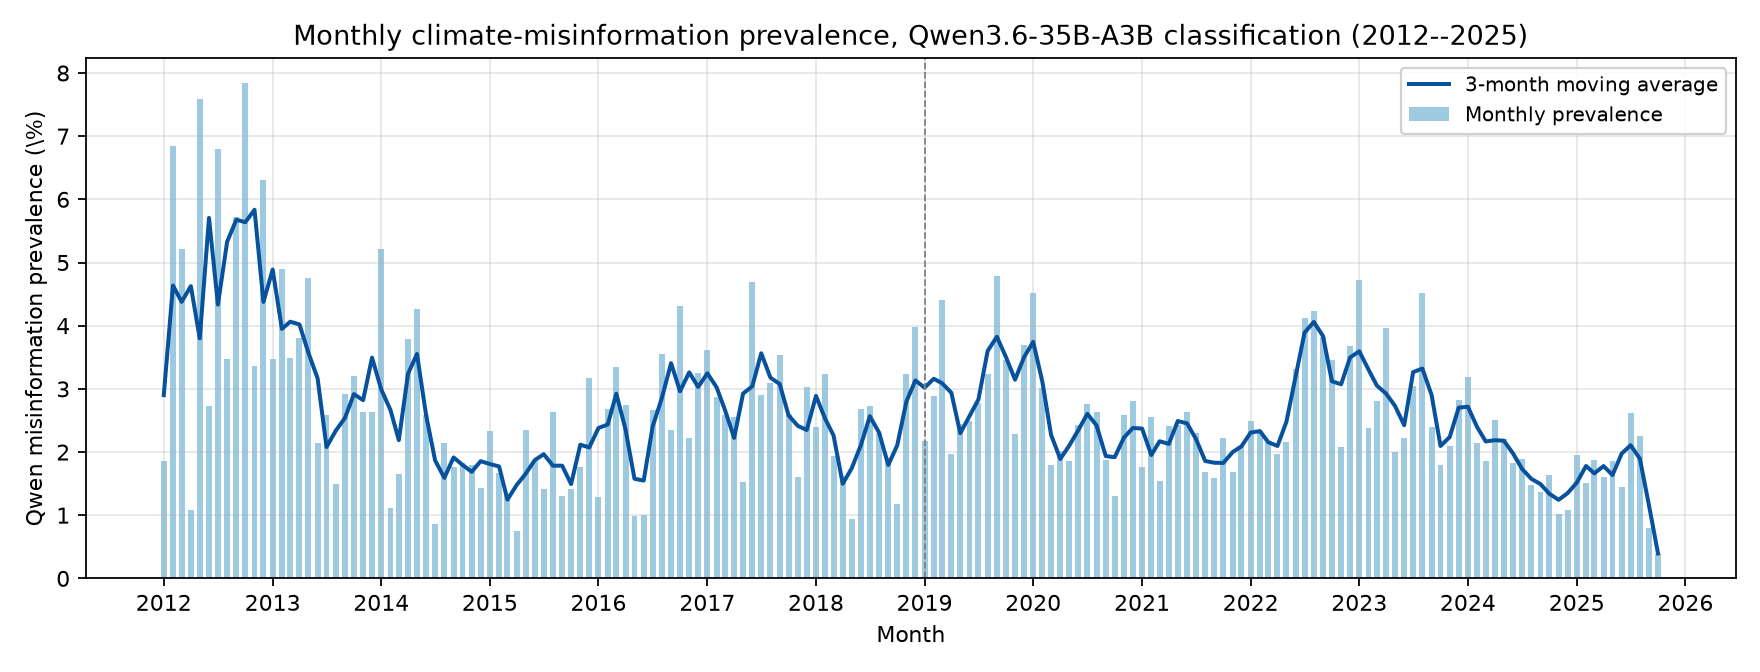
\includegraphics[width=\linewidth]{figures/fig_v2_qwen_prevalence_ts.png}
\caption{Monthly climate-misinformation prevalence in the Qwen3.6-35B-A3B classification, 2012--2025. Bars are monthly prevalence (flagged posts as a share of that month's paired posts); the solid line is a three-month moving average. The dashed line marks January 2019.}
\label{fig:qwen_prevalence_ts}
\end{figure}

\begin{figure}[!ht]
\centering
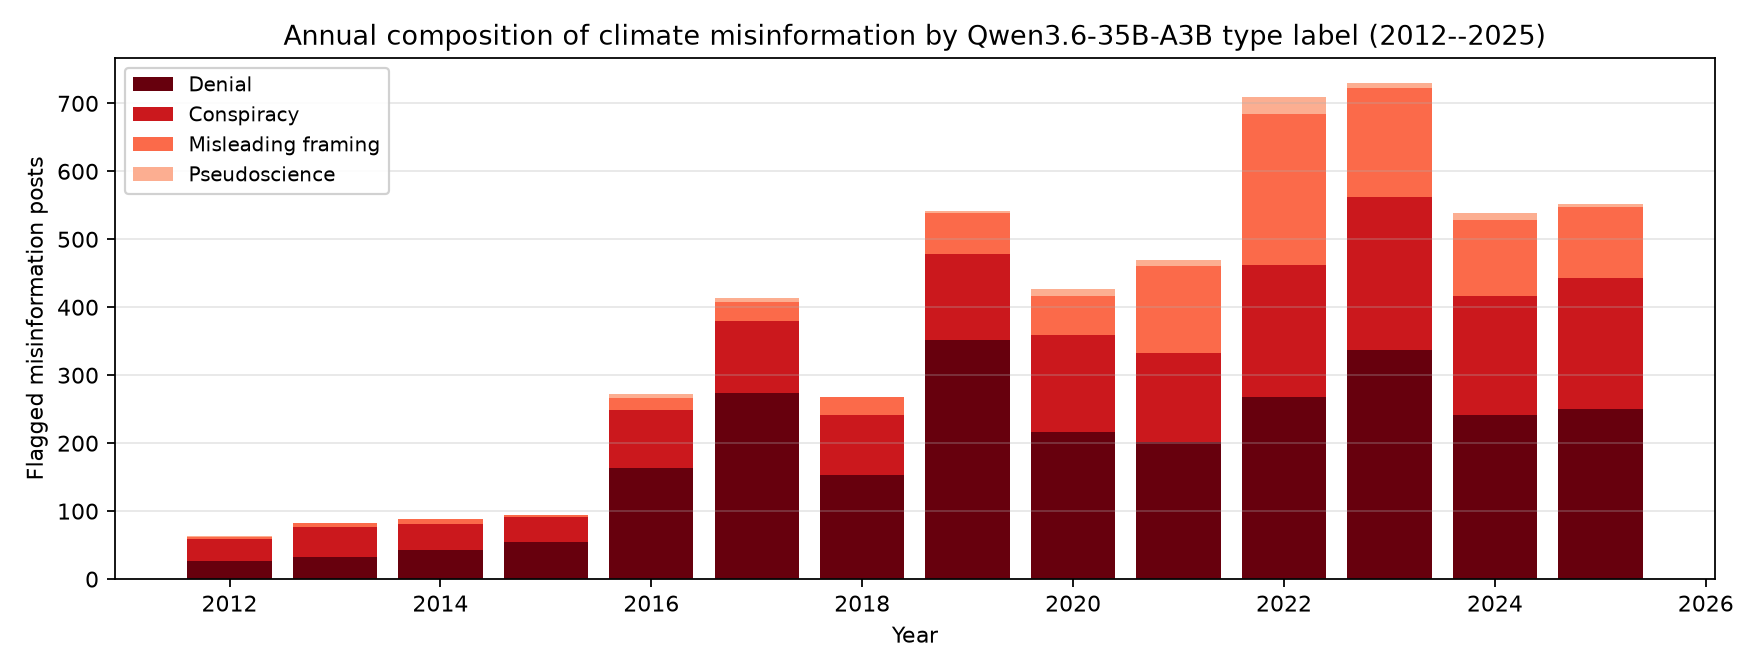
\includegraphics[width=\linewidth]{figures/fig_v2_qwen_type_composition.png}
\caption{Annual composition of Qwen-classified climate misinformation by type, 2012--2025. Denial and conspiracy framings account for the bulk of flagged content and for its post-2019 growth.}
\label{fig:qwen_type_composition}
\end{figure}

\FloatBarrier
\section{Network Structure of Misinformation Dissemination}
\label{sec:appendix_network}

I supplement the post-level corpus with an owner-based network constructed on the 150 most active and engaged post owners (pages and profiles), selected via a composite ranking weighting total engagement (40\%), misinformation post count (40\%), and overall posting activity (20\%). Two owners are connected if their monthly posting distributions correlate at $\rho \geq 0.3$ (Pearson). The largest connected component contains 142 nodes and 1{,}004 edges, with five Louvain communities (\cite{blondel2008louvain}) of community misinformation rates varying from 4.2\% to 21.7\%. The threshold captures accounts that post more during the same months, which may reflect coordinated dissemination, shared thematic interests, or common responses to COP meetings, extreme weather, or elections; the network structure should therefore be read as thematic co-occurrence rather than necessarily coordinated inauthentic behaviour (\cite{walter2020evaluating}; \cite{williams2015network}).

Three centrality measures bear on the empirical specification that follows. Eigenvector centrality is negatively correlated with the per-owner misinformation rate ($r = -0.296$, $p = 0.0004$), and degree centrality is positively correlated with the absolute misinformation count ($r = 0.218$, $p = 0.009$); betweenness centrality shows no significant association ($r = -0.068$, $p = 0.42$). The structurally central nodes disseminate proportionally lower rates of misleading content, while peripheral high-degree nodes generate larger absolute volumes. This pattern weakens, rather than supports, the prior assumption that engagement-weighting captures ``reach-amplified misinformation'': if reach were dominated by misinformation-heavy actors, eigenvector centrality should covary positively, not negatively, with misinformation rate.  Figures~\ref{fig:network_main} and~\ref{fig:centrality_misinfo} display the network and centrality scatterplots respectively.

\begin{figure}[!ht]
\centering
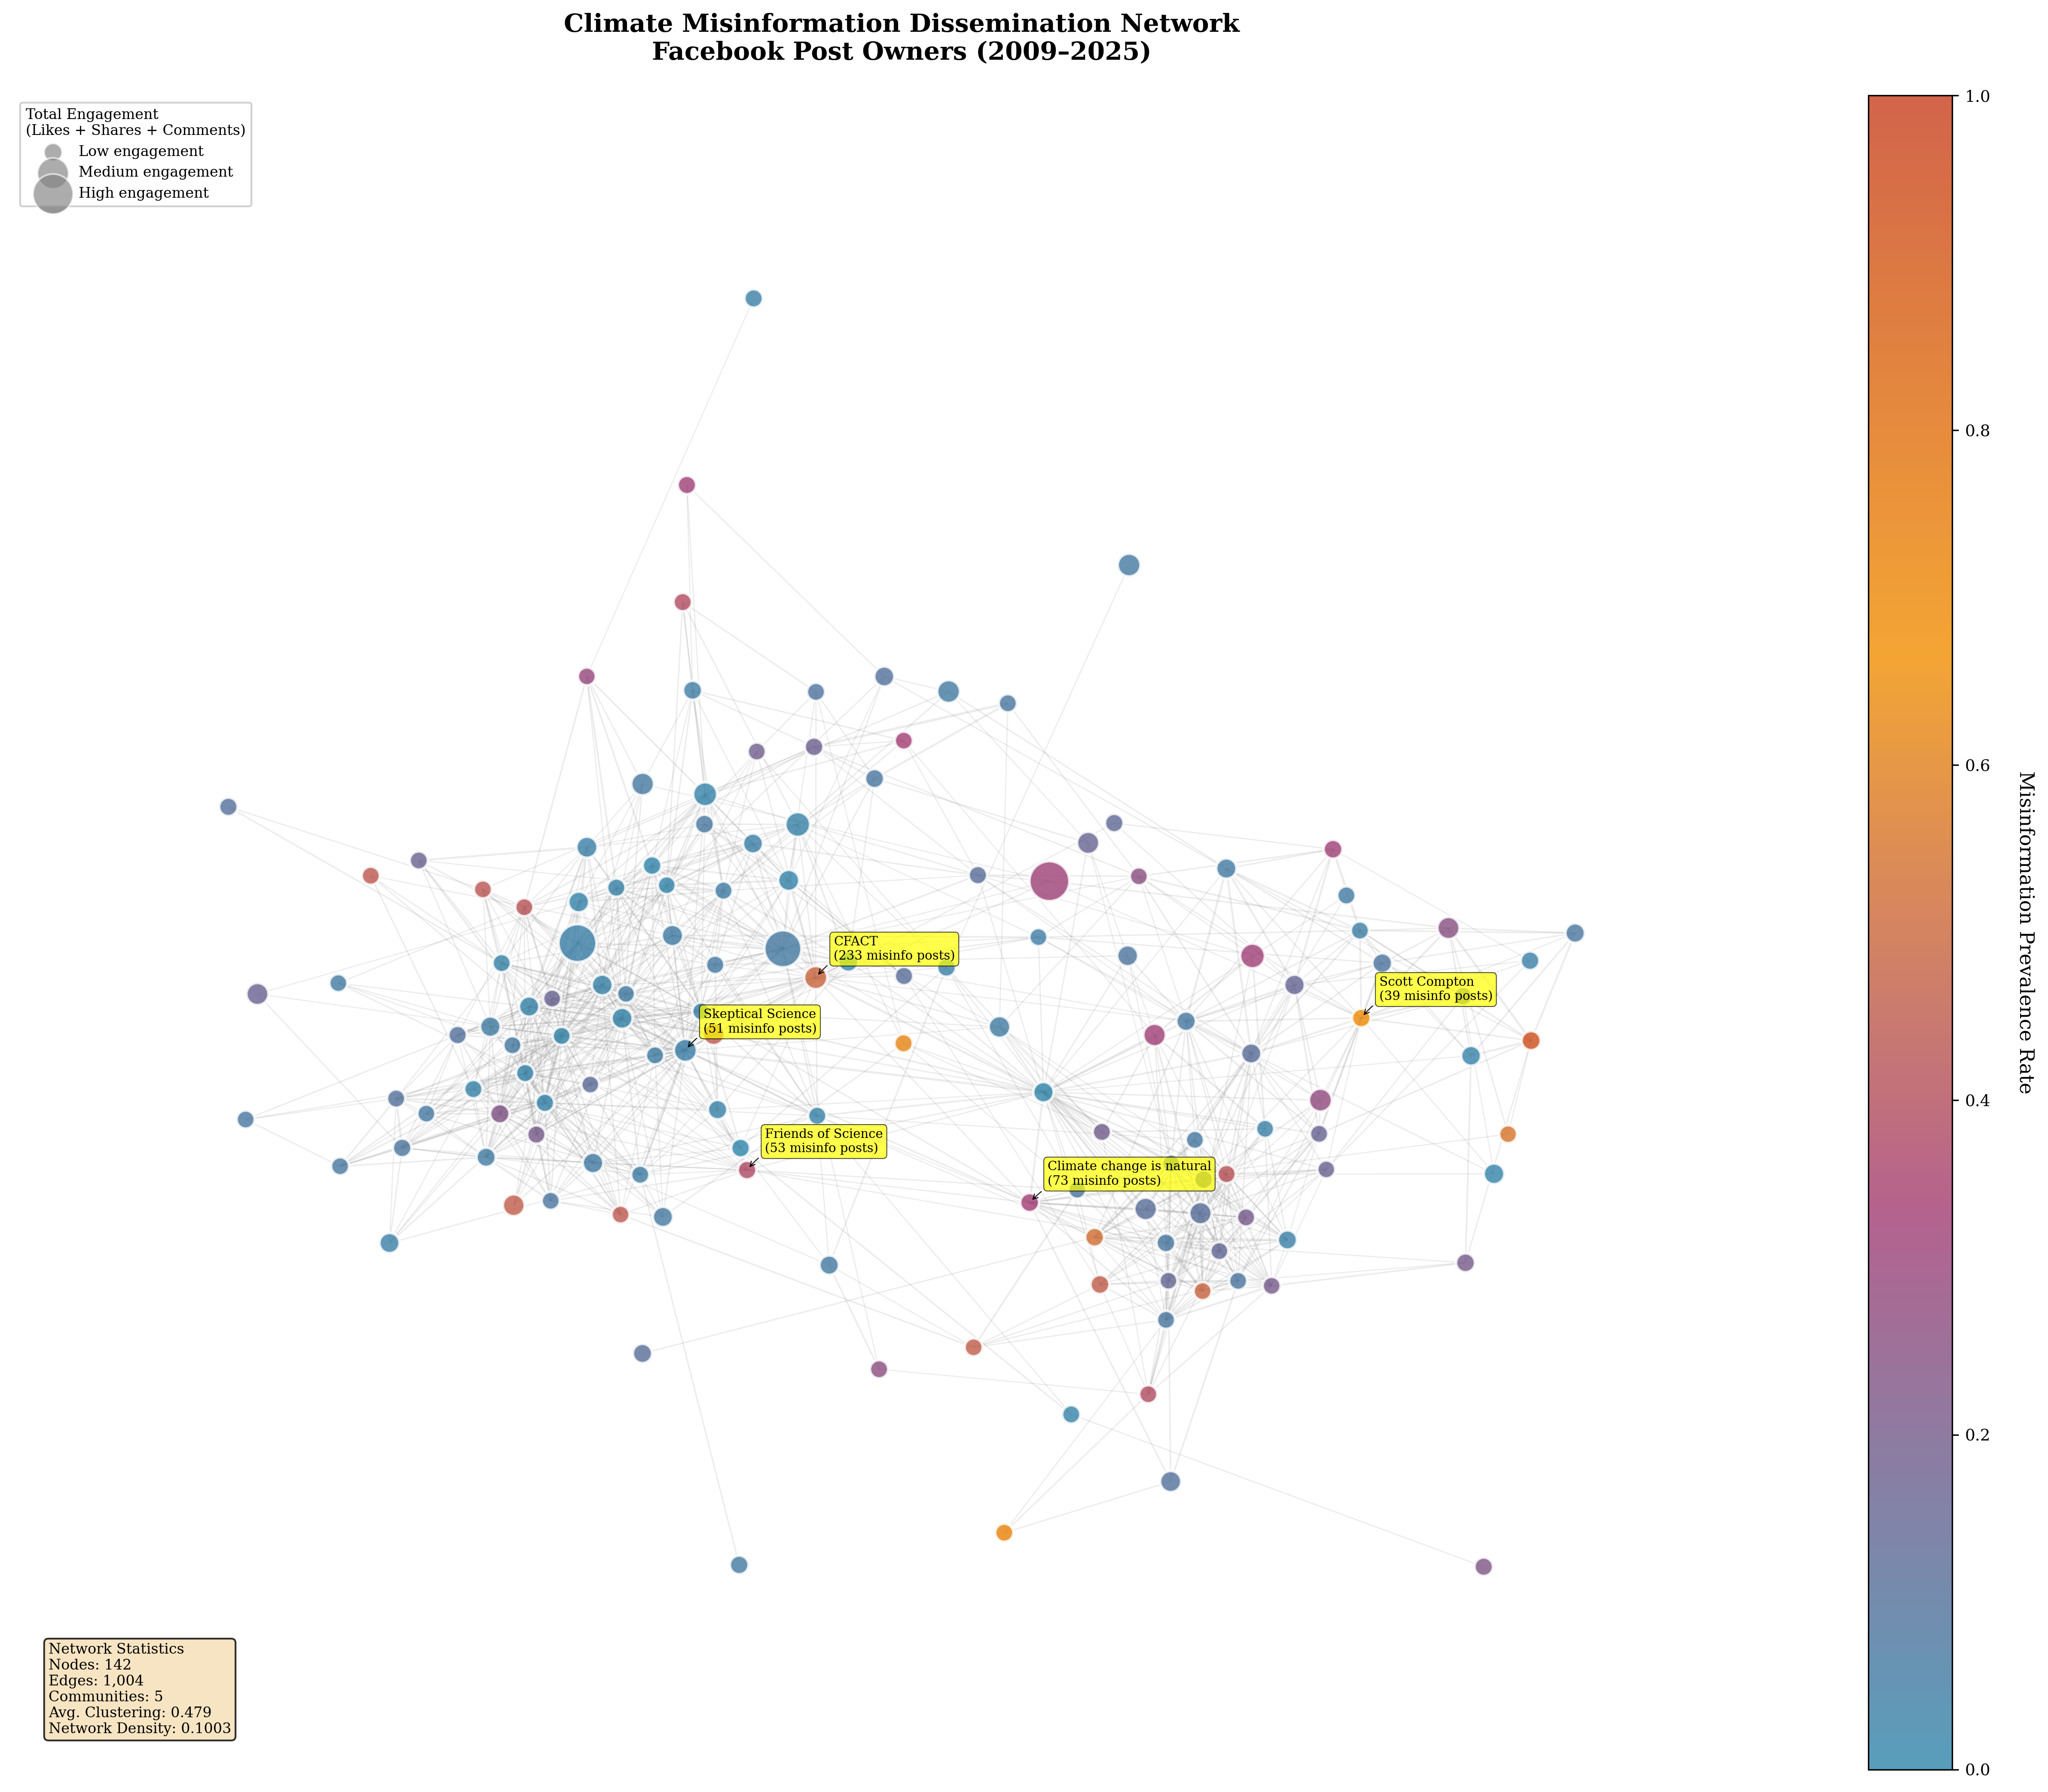
\includegraphics[width=\textwidth]{climate_misinfo_network.png}
\caption{Climate Misinformation Dissemination Network}
\label{fig:network_main}
\begin{minipage}{\textwidth}
\small
\textit{Notes:} Network graph of 142 Facebook post owners (pages/profiles) constructed from temporal posting correlations (Pearson $\rho \geq 0.3$). Node size is proportional to total engagement (likes + shares + comments). Node color indicates misinformation prevalence rate (blue = low, red = high). Edge thickness reflects correlation strength. Top 5 misinformation spreaders are labeled. Force-directed layout (Fruchterman--Reingold). Network statistics: 5 communities (Louvain), average clustering = 0.48, density = 0.10. Data source: Meta Content Library, Dec 2009-Oct 2025.
\end{minipage}
\end{figure}

\begin{figure}[!ht]
\centering
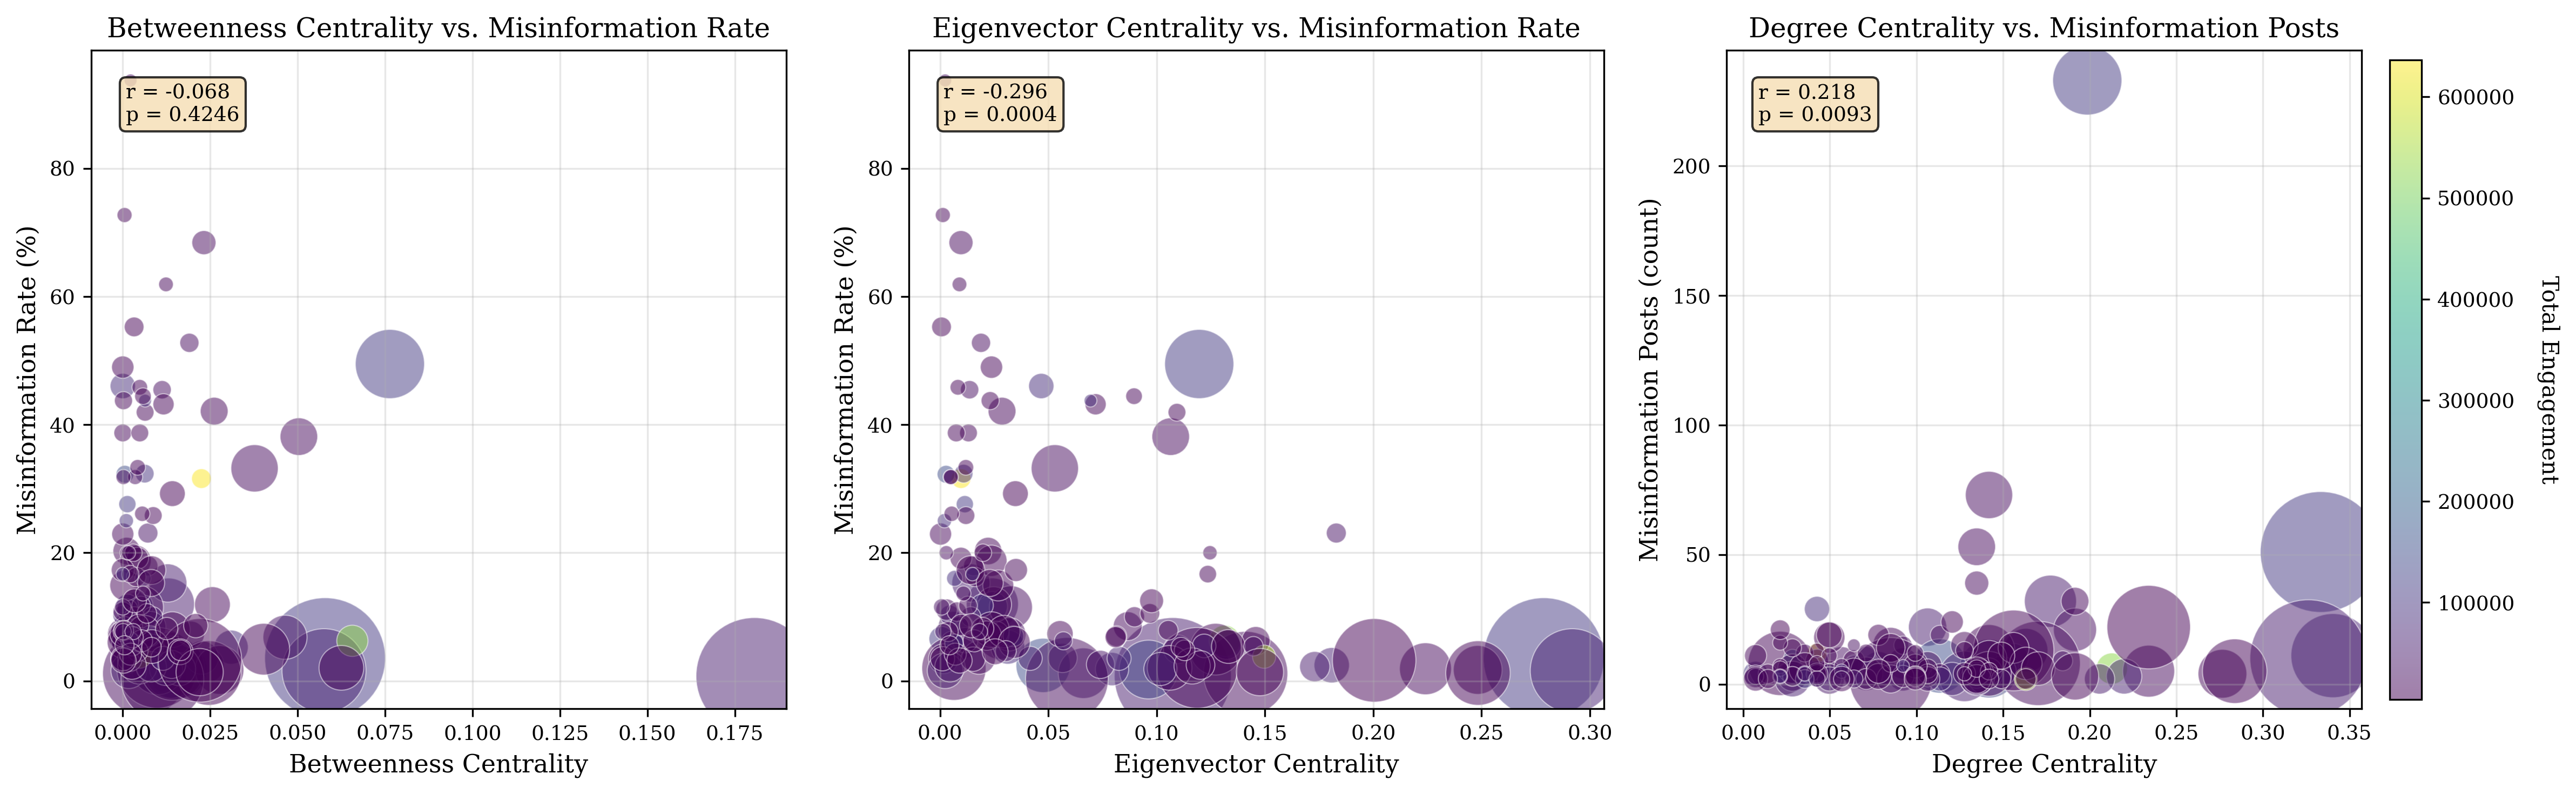
\includegraphics[width=\textwidth]{validation_test.png}
\caption{Network Centrality and Misinformation Prevalence}
\label{fig:centrality_misinfo}
\begin{minipage}{\textwidth}
\small
\textit{Notes:} Scatterplots of three centrality measures against misinformation prevalence and count. \textbf{Left panel:} Betweenness centrality vs. misinformation rate ($r = -0.068$, $p = 0.42$). \textbf{Center panel:} Eigenvector centrality vs. misinformation rate ($r = -0.296$, $p = 0.0004$). \textbf{Right panel:} Degree centrality vs. misinformation post count ($r = 0.218$, $p = 0.009$). Node size represents total posts. Color indicates total engagement. Eigenvector centrality exhibits a statistically significant negative association with misinformation rate, suggesting influential nodes spread less misinformation.
\end{minipage}
\end{figure}

\FloatBarrier
\section{Firm-Day Exposure: Descriptive Statistics and Validation}
\label{sec:firmday_validation}

This appendix reports the descriptive statistics of the firm-day misinformation-exposure
index introduced in Section~\ref{sec:LLM} and the held-out spot-check used to validate
the classifier's handling of satire and politically loaded but non-climate content.

\subsection{Descriptive Statistics}
Table~\ref{tab:v2_descriptive} summarises the firm-day index and its constituent scores
across the 714,227 firm-days in the climate-transition panel with at least one paired
post. The index $\mathrm{Exp}^{\text{mean}}_{i,t}$ has a mean of $0.34$ on a 0--100 scale,
a median of $0.09$, a 99th percentile of $2.73$, and a share of exactly-zero firm-days of
$44\%$. The sum variant $\mathrm{Exp}^{\text{sum}}_{i,t}$ has mean $21.85$ and 99th
percentile $171.50$; the log-transformed version $\log(1+\mathrm{Exp}^{\text{sum}}_{i,t})$
is approximately normal in shape with mean $1.80$ and 99th percentile $5.15$. The
misinformation sub-score $M^{\text{mean}}_{i,t}$ has mean $1.73$, p99 $15.60$, and a share
of exactly-zero firm-days of $41\%$, reflecting the rubric's restriction of
misinformation scoring to climate-or-energy claims. The relevance sub-score
$R^{\text{mean}}_{i,t}$ has mean $12.59$ and p99 $27.17$, with only $2\%$ of firm-days
exactly at zero, indicating that climate posts paired by date are typically at least
weakly relevant to the firm's sub-industry.

\begin{table}[htbp]
\centering
\caption{Descriptive statistics of the firm-day misinformation-exposure IV (climate-transition panel, 714,227 firm-days with $\geq 1$ climate post)}
\label{tab:v2_descriptive}
\begin{threeparttable}
\begin{tabular}{l r r r r r r}
\toprule
Variable & Mean & SD & $p_{50}$ & $p_{90}$ & $p_{99}$ & Share zero \\
\midrule
\# climate posts paired to the firm-day & 59.900 & 49.449 & 52.000 & 127.000 & 208.000 & 0.017 \\
Mean per-post sector relevance $R^{\text{mean}}$ & 12.594 & 5.106 & 12.231 & 18.524 & 27.173 & 0.022 \\
Mean per-post climate misinformation $M^{\text{mean}}$ & 1.731 & 3.232 & 0.781 & 4.268 & 15.600 & 0.408 \\
Firm-day mean exposure $\mathrm{Exp}^{\text{mean}}$ & 0.338 & 0.715 & 0.090 & 0.971 & 2.732 & 0.442 \\
Firm-day max exposure $\mathrm{Exp}^{\text{max}}$ & 13.526 & 20.236 & 7.000 & 50.700 & 68.640 & 0.442 \\
Firm-day sum exposure $\mathrm{Exp}^{\text{sum}}$ & 21.846 & 37.661 & 7.500 & 71.250 & 171.500 & 0.442 \\
Share of posts with $M\geq 25$ & 0.020 & 0.037 & 0.009 & 0.050 & 0.167 & 0.464 \\
$\log(1+\mathrm{Exp}^{\text{sum}})$ & 1.795 & 1.758 & 2.140 & 4.280 & 5.150 & 0.442 \\
\bottomrule
\end{tabular}
\begin{tablenotes}\small
\item \textit{Notes:} Sample is firm-days in the energy panel for which at least one English-language Facebook
climate post on the same calendar date was scored against the firm's TRBC industry. ``Share zero'' is the
fraction of firm-days for which the variable evaluates to exactly 0 (typically because no posts in the day's
classification batch were judged sector-relevant or misinformation-laden).
\end{tablenotes}
\end{threeparttable}
\end{table}

Figure~\ref{fig:v2_iv_distribution} plots the distribution of the headline index and
its log-volume variant on non-zero firm-days. The mean variant has a long right tail
truncated by the bound of the 0--100 scale; the log-volume variant is more
symmetric, justifying its use in the variant Model~I specification reported in
Table~\ref{tab:v2_core}.

\begin{figure}[!ht]
\centering
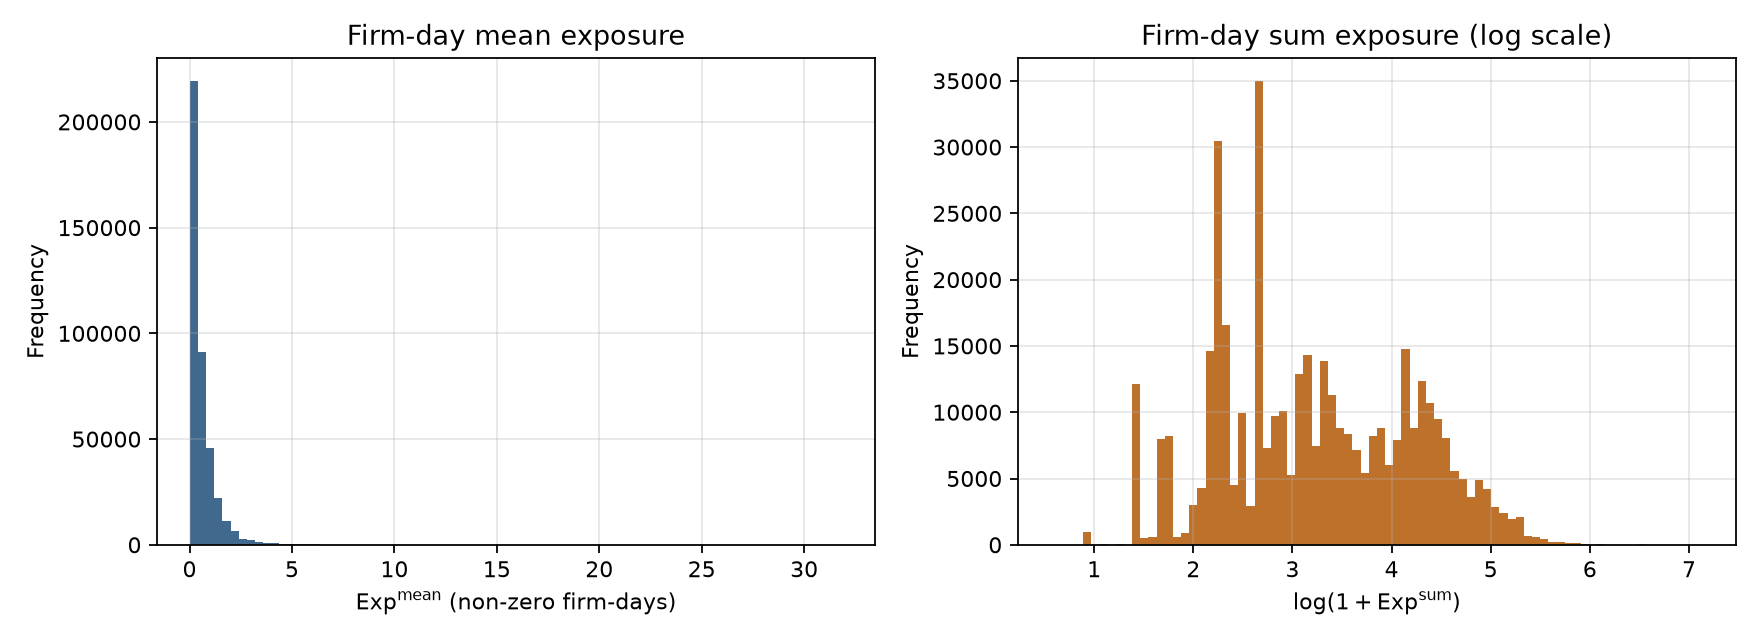
\includegraphics[width=\linewidth]{figures/fig_v2_iv_distribution.png}
\caption{Firm-day exposure distribution. Left panel: $\mathrm{Exp}^{\text{mean}}_{i,t}$
on non-zero firm-days. Right panel: $\log(1+\mathrm{Exp}^{\text{sum}}_{i,t})$.}
\label{fig:v2_iv_distribution}
\end{figure}

\subsection{Classifier Validation}
The classifier was validated on a held-out spot-check of the first 2,000 (post,
sub-industry) judgments. Two qualitative findings shaped the final rubric. First, a
default rubric (``score climate misinformation on a continuous 0--100 scale'')
over-scored politically charged but non-climate content. Anti-vaccine conspiracy
posts, antisemitic content about EU politicians, and electoral-fraud posts that
happened to be paired to climate sub-industries by calendar date received high
misinformation scores under the default rubric despite making no empirical claims
about climate or energy. The headline composite $\mathrm{Exp}_{p,s}=R_{p,s}\cdot
M_{p,s}/100$ partially neutralised this leakage because relevance scores on
sector-irrelevant content were low, but the misinformation sub-score itself was
contaminated. The final rubric (Section~\ref{sec:LLM}) explicitly restricts
misinformation scoring to climate-or-energy claims, and a re-run of the spot-check
under the final rubric produced misinformation scores of zero on the politically
charged but non-climate items.

Second, sarcastic and parodic content that mocked climate denial received high
misinformation scores under the default rubric. A representative example begins
``MDPI, the predatory journal of which nothing can be believed, according to
Facebook climate experts, recently published a dubious study on anthropogenic
warming\ldots'' and ends with the parody credit ``A DONT BELIEVE EVERYTHING YOU
READ PRODUCTION''. The default rubric scored this post at $M_{p,s}=95$ with the
type label ``denial''; the final rubric, which includes an explicit instruction to
treat satire and parody as not-misinformation, scores it at $M_{p,s}=0$ with the
rationale ``satirical parody mocking climate denialism, not a sincere assertion of
false claims''. Both rubric refinements were committed to the spec before the
production run, and the production run used the final rubric.

\subsection{Within-Classifier Placebo}
Section~\ref{sec:results_placebo} reports a within-classifier placebo built from
the subset of posts whose per-post sector-relevance score $R_{p,s}<10$. The
placebo aggregates the same exposure measure across only the posts the classifier
identified as off-topic for the firm's sub-industry; under the empirical
strategy of Section~\ref{sec:model}, that aggregate should not move the firm-day
outcomes if the headline effect is climate-specific. The placebo coefficients on
Models I--III are statistically indistinguishable from zero
(Table~\ref{tab:v2_placebo}), which supports the climate-specific
interpretation without establishing it.

\FloatBarrier
\section{Heterogeneity and Interaction Checks}
\label{sec:appendix_heterogeneity}

\subsection{Renewable--Fossil, Regional, and Temporal Splits}
\label{sec:results_signflip}

Table~\ref{tab:v2_signflip} estimates the three models on the renewable and fossil sub-panels, on each of the five regions, and on the pre/post-2019 samples, using $\mathrm{Exp}^{\text{mean}}$ under two-way clustering. Figure~\ref{fig:v2_signflip_coef} plots the same coefficients with 95\% confidence intervals.

\begin{table}[htbp]
\centering
\caption{Climate-Transition Panel: Coefficient Heterogeneity across Renewable--Fossil, Regional, and Temporal Splits (Two-Way Clustered SE)}
\label{tab:v2_signflip}
\begin{threeparttable}
\begin{tabular}{l r r r r r r}
\toprule
 & \multicolumn{2}{c}{Model I: Spread\%} & \multicolumn{2}{c}{Model II: CAPM $\beta$} & \multicolumn{2}{c}{Model III: ExcessReturn} \\
\cmidrule(lr){2-3}\cmidrule(lr){4-5}\cmidrule(lr){6-7}
Subsample & Coef. & $N$ & Coef. & $N$ & Coef. & $N$ \\
\midrule
Renewables & +0.0046 & 76,680 & -0.0012 & 56,892 & -0.0417 & 56,678 \\
Fossil fuels & +0.0028 & 391,382 & -0.0006 & 327,125 & -0.0180 & 326,212 \\
United States & +0.0077 & 219,693 & +0.0008 & 160,380 & -0.0102 & 157,825 \\
United Kingdom & -0.0010 & 6,954 & -0.0014 & 4,283 & +0.0190 & 4,297 \\
European Union & -0.0005 & 4,802 & +0.0050 & 4,556 & +0.0307 & 4,678 \\
China & +0.0007 & 194,377 & -0.0016 & 175,484 & -0.0443 & 176,846 \\
Japan & +0.0034 & 42,236 & -0.0035$^{***}$ & 39,314 & +0.0085 & 39,244 \\
Pre-2019 & -0.0005 & 193,062 & +0.0014 & 157,871 & -0.0240 & 164,801 \\
Post-2019 & +0.0056$^{**}$ & 275,000 & -0.0077$^{***}$ & 226,146 & -0.0039 & 218,088 \\
\bottomrule
\end{tabular}
\begin{tablenotes}\small
\item \textit{Notes:} Each cell is the OLS coefficient on $\mathrm{Exp}^{\text{mean}}$ in the
specification of Table~\ref{tab:v2_core}, estimated on the indicated subsample of the energy panel.
Standard errors are clustered on RIC and Date. Cells where $N<1{,}000$ are omitted.
$^{*}p<0.10$, $^{**}p<0.05$, $^{***}p<0.01$.
\end{tablenotes}
\end{threeparttable}
\end{table}

\begin{figure}[htbp]
\centering
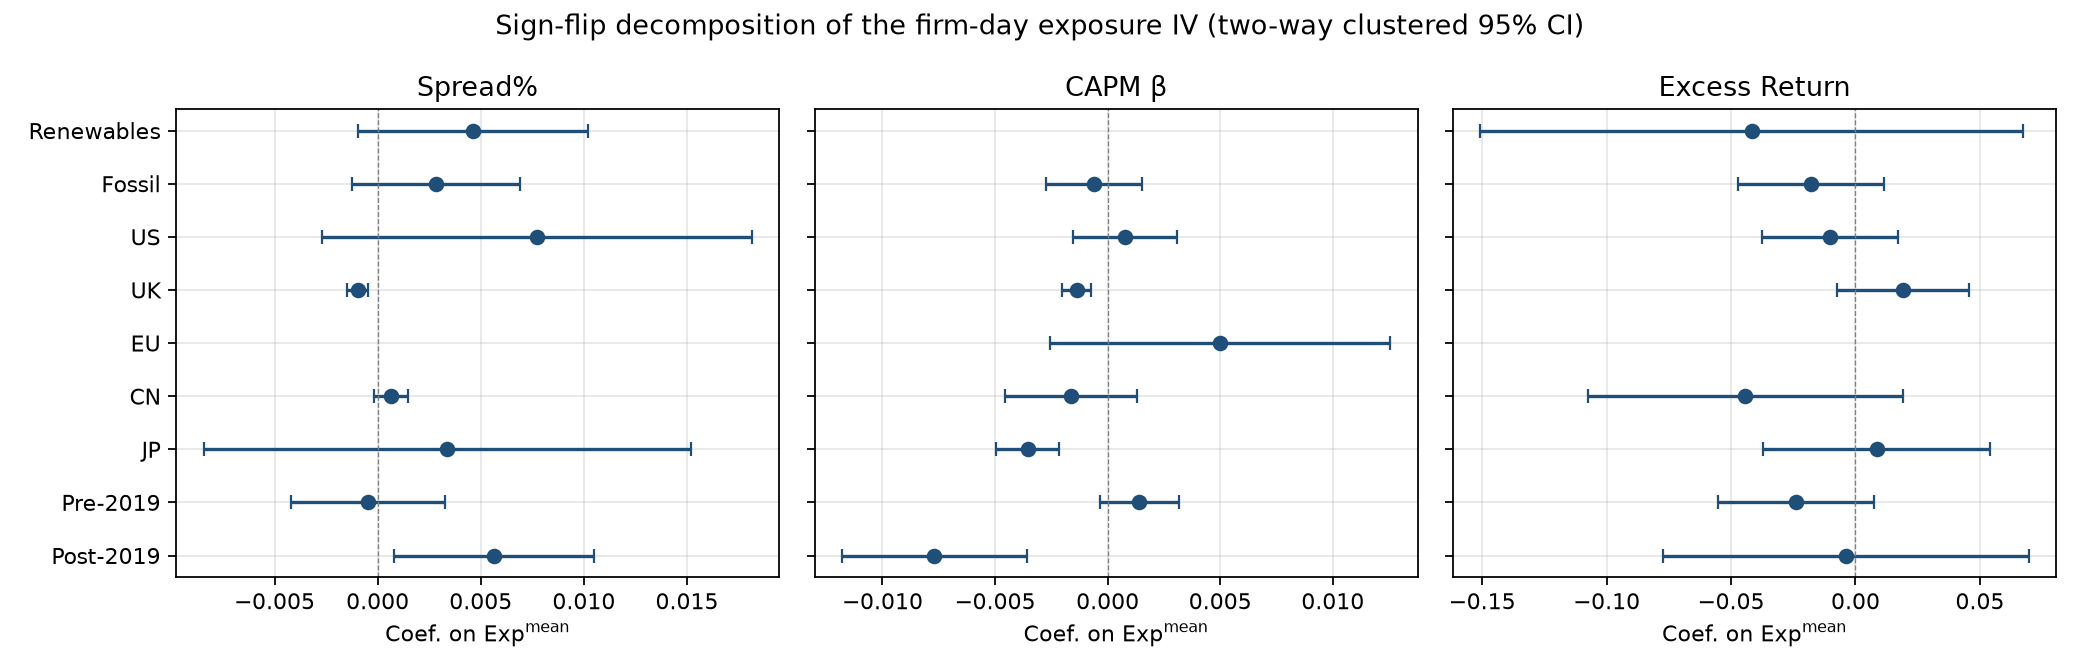
\includegraphics[width=\linewidth]{figures/fig_v2_signflip_coef.png}
\caption{Heterogeneity of the firm-day exposure coefficient across renewable/fossil, regional, and pre/post-2019 splits, by model. Markers are coefficients on $\mathrm{Exp}^{\text{mean}}_{i,t}$; horizontal bars are two-way clustered (RIC + Date) 95\% confidence intervals. The post-2019 cell carries the strongest Model I and Model II signals.}
\label{fig:v2_signflip_coef}
\end{figure}

The temporal split is discussed in Section~\ref{sec:results_subperiod}; it is reproduced here so that the renewable--fossil, regional, and subperiod estimates can be compared in a common figure.

The regional and renewable--fossil comparisons are less precise. The US Model~I coefficient is positive but not significant ($+0.0077$, $p=0.15$), while the UK and EU estimates have small samples. The fossil-only and renewable-only Model~I coefficients are both positive ($+0.0028$, $p=0.17$ and $+0.0046$, $p=0.11$), and their difference is not significant. The data therefore do not show that the spread response is cleanly divided between fossil and renewable firms.

\subsection{Exploratory Triple Interaction}
\label{sec:results_triple}

Table~\ref{tab:v2_triple} interacts $\mathrm{Exp}^{\text{mean}}_{i,t}$ with Fossil-sub-industry, English-region (US or UK), and Post-2019 indicators in the Model~I specification.

\begin{table}[htbp]
\centering
\caption{Triple interaction: Fossil $\times$ English-region $\times$ Post-2019 (Model~I, Spread\%, two-way clustered SE)}
\label{tab:v2_triple}
\begin{threeparttable}
\begin{tabular}{l r r}
\toprule
Term & Coef. & SE \\
\midrule
$\mathrm{Exp}^{\text{mean}}$ & +0.0049 & (0.0192) \\
$\mathrm{Exp}^{\text{mean}}\!\times\!\mathbb{1}\{\text{Fossil}\}$ & -0.0067 & (0.0205) \\
$\mathrm{Exp}^{\text{mean}}\!\times\!\mathbb{1}\{\text{English region}\}$ & -0.1525$^{*}$ & (0.0862) \\
$\mathrm{Exp}^{\text{mean}}\!\times\!\mathbb{1}\{\text{Post-2019}\}$ & -0.0125 & (0.0404) \\
$\mathrm{Exp}^{\text{mean}}\!\times\!\text{Fossil}\!\times\!\text{English}$ & +0.1499$^{*}$ & (0.0870) \\
$\mathrm{Exp}^{\text{mean}}\!\times\!\text{Fossil}\!\times\!\text{Post-2019}$ & -0.0010 & (0.0483) \\
$\mathrm{Exp}^{\text{mean}}\!\times\!\text{English}\!\times\!\text{Post-2019}$ & +0.3624$^{*}$ & (0.1925) \\
$\mathrm{Exp}^{\text{mean}}\!\times\!\text{Fossil}\!\times\!\text{English}\!\times\!\text{Post-2019}$ & -0.2930 & (0.1987) \\
\midrule
$N$ & 468,062 & \\
\bottomrule
\end{tabular}
\begin{tablenotes}\small
\item \textit{Notes:} Estimation by Model~I; controls and fixed effects as in
Table~\ref{tab:v2_core}. ``English region'' is US or UK. ``Fossil'' identifies the seven fossil
TRBC sub-industries; ``Renewable'' firms are the complement within the energy panel.
$^{*}p<0.10$, $^{**}p<0.05$, $^{***}p<0.01$.
\end{tablenotes}
\end{threeparttable}
\end{table}

The three-way interaction is difficult to interpret and is not statistically significant at conventional levels. Two terms are marginal: $\mathrm{Exp}\times\text{English}$ at $p=0.078$ and $\mathrm{Exp}\times\text{English}\times\text{Post-2019}$ at $p=0.061$. These estimates are treated as exploratory because the interaction divides the 204-firm sample into small cells and does not identify the coefficients precisely. The simpler subperiod and regional comparisons provide the more interpretable evidence.

\FloatBarrier
\section{Summary}

The appendix consolidates the descriptive and diagnostic evidence behind the paper's design. The corpus tables document the scale, heterogeneity, and engagement structure of the Facebook data; the network section maps the dissemination structure of the most active post owners. Together they document how the explanatory variable is constructed from variation in post volume, engagement, and timing.

The financial and exposure sections document the breadth and stability of the financial panel, the composition of the climate-transition subsample, and the construction of the firm-day exposure index itself: its distributional properties, the held-out spot-check that fixed the classification rubric before the production run, and the within-classifier placebo. Read as a whole, the appendix connects the competing-liquidity framework of Section~\ref{sec:theory} to the empirical results in Section~\ref{sec:results}.

\end{document}
